\chapter{概率论}
\label{chap:probability-theory}

前两部分研究的对象即使很复杂，给定输入后仍有确定结果。现在考虑一个不同的问题：传感器反复测量同一信号，读数却会受到噪声扰动；学习算法面对有限候选模型，也只能依据有限样本
比较它们。单次结果无法代表整体规律，而“多测几次再平均”又留下三个问题：平均的对象是什么，观测增加时平均是否稳定，以及从多个候选中挑出表现最好的一个后，原有误差保证是否仍然成立。

概率论用测度描述结果的不确定性，用积分定义平均，并用条件化表达信息增加后的判断。本章复用第~\ref{chap:mathematical-analysis}章的测度、积分与极限工具，不再重证单调收敛、
支配收敛和Fubini定理。我们从有限概率表进入一般概率空间，再沿密度比和条件期望说明“改变分布”与“增加信息”的区别。随后，带噪观测的样本平均贯穿随机收敛、蒙特卡洛
估计和集中不等式；有限候选的比较则把单个平均的误差推广为同时误差。章末还会看到，有些有限样本保证不依赖独立性，而来自观测次序的对称性。

\section{概率表示与条件化}
\label{sec:probability-representation-conditioning}

本科概率论中的概率表、密度和条件平均，在一般样本空间中需要一个共同框架。
本节先复用测度与积分表示分布，再区分改变参考测度和增加可用信息两种操作。
独立性则是联合分布的额外条件，不能由边缘分布或不相关性代替。
这些条件会直接决定后面哪些抽样误差工具可用。

\subsection{概率空间与随机变量}
\label{sec:probability-spaces-random-variables}

\subsubsection{有限概率表与事件测度}

设一次带噪观测只能取有限个结果\(\Omega=\{\omega_1,\ldots,\omega_m\}\)，并为每个结果指定权重\(p_j\geq0\)，满足\(\sum_{j=1}^{m}p_j=1\)。事件
\(A\subseteq\Omega\)的概率为
\[ \mathbb{P}(A)=\sum_{\omega_j\in A}p_j. \]
这个有限公式已经包含三条基本规则：概率非负，全集概率为\(1\)，互不相交事件的概率可以相加。一般样本空间可能不可数，而且未必希望给每个子集都赋概率。第~\ref{chap:mathematical-analysis}章的测度语言恰好把这三条规则推广到这种情形。

\begin{definition}[概率空间]
  \label{def:probability-space}
\term{概率空间}（probability space）是三元组\((\Omega,\mathcal{F},\mathbb{P})\)。其中，\(\Omega\)是所有可能结果组成的
样本空间，\(\mathcal{F}\)是事件组成的\(\sigma\)代数，\(\mathbb{P}:\mathcal{F}\to[0,1]\)是满足
\(\mathbb{P}(\Omega)=1\)的测度。可数可加性说明，对两两不交的事件\((A_j)_{j\geq1}\)，
\[ \mathbb{P}\left(\bigcup_{j\geq1}A_j\right)
  =\sum_{j\geq1}\mathbb{P}(A_j). \]
\end{definition}
概率不是附着在口头描述上的数，而是定义在指定事件族上的测度。若改变\(\mathcal{F}\)，能够询问的事件也会改变。

对事件\(A\)，其补事件和单调性分别给出
\[ \mathbb{P}(A^{\mathsf c})=1-\mathbb{P}(A),
  \qquad A\subseteq B\Longrightarrow\mathbb{P}(A)\leq\mathbb{P}(B). \]
概率测度还与单调极限相容。若\(A_n\uparrow A\)，令
\(B_1=A_1\)、\(B_n=A_n\setminus A_{n-1}\)，则\((B_n)\)两两不交且
\(A=\bigcup_nB_n\)。可数可加性因而给出
\[
  \mathbb{P}(A)
  =\sum_{n\geq1}\mathbb{P}(B_n)
  =\lim_{n\to\infty}\mathbb{P}(A_n).
\]
若\(A_n\downarrow A\)，对补事件使用上一结论便得到
\(\mathbb{P}(A_n)\to\mathbb{P}(A)\)。第二个结论用到了
\(\mathbb{P}(A_1)\leq1<\infty\)；对一般无限测度，递减连续性必须另外要求起始集合具有有限测度。

对任意可数事件族，即使事件不互斥，也有联合界
\begin{equation}
  \mathbb{P}\left(\bigcup_{j\geq1}A_j\right)
  \leq
  \sum_{j\geq1}\mathbb{P}(A_j).
  \label{eq:probability-union-bound}
\end{equation}
第~\ref{sec:probability-random-functions-uniform-error}节会用它同时控制有限候选的误差。

\subsubsection{随机变量与分布}

\begin{definition}[随机变量]
  \label{def:probability-random-variable}
给定可测空间\((\mathcal{X},\mathcal{A})\)，若映射
\(X:\Omega\to\mathcal{X}\)满足
\(X^{-1}(B)\in\mathcal{F}\)对每个\(B\in\mathcal{A}\)成立，就称\(X\)为取值于
\(\mathcal{X}\)的\term{随机变量}（random variable）。
\end{definition}
对实值变量，只需验证
\[ \{\,\omega:X(\omega)\leq x\,\}\in\mathcal{F},
  \qquad x\in\mathbb{R}, \]
因为这些半无限区间生成\(\mathcal{B}(\mathbb{R})\)。可测性保证由取值范围定义的
原像确实属于\(\mathcal{F}\)，因而有概率。随机变量不是“本身会随机变化的符号”，而是把基础结果转换成所关心对象的可测函数。

\(X\)在实数轴上诱导的概率测度称为它的\term{分布}（distribution）：
\[ \mathbb{P}_X(B)
  =\mathbb{P}(X\in B),\qquad B\in\mathcal{B}(\mathbb{R}). \]
分布函数
\[ F_X(x)=\mathbb{P}(X\leq x) \]
单调不减、右连续，并满足\(\lim_{x\to-\infty}F_X(x)=0\)与\(\lim_{x\to\infty}F_X(x)=1\)。反过来，每个具有这些性质的函数都对应某个实随机变量的分布。

若\(\mathbb{P}_X\)集中在可数点集上，可写成概率质量函数\(p_X(x)=\mathbb{P}(X=x)\)。若它相对于Lebesgue测度有密度\(f_X\)，则
\[ \mathbb{P}(X\in B)=\int_B f_X(x)\,\mathrm{d}x,
  \qquad F_X(x)=\int_{-\infty}^{x}f_X(t)\,\mathrm{d}t. \]
密度值不是单点概率。连续分布通常满足\(\mathbb{P}(X=x)=0\)，但
\(f_X(x)\)仍可为正；在密度连续的点，它等于小邻域概率除以邻域长度后的局部极限；一般密度只在几乎处处意义下确定，不能在任意指定点都作这样的解释。
例如\(X\)在区间\([0,1/4]\)上均匀分布时，\(f_X(x)=4\mathbb{I}\{0\leq x\leq1/4\}\)。
密度值\(4\)可以大于\(1\)，因为概率由面积而非高度给出：
\(\mathbb{P}(0.10\leq X\leq0.15)=4\times0.05=0.2\)，而每个单点的概率仍为\(0\)。

图~\ref{fig:probability-density-cdf}把这一区分放在同一个分布上：密度图中的矩形面积，正是分布函数在区间两端的增量。因而从分布函数求区间概率不需要把连续结果变成单点概率。

\begin{figure*}[htbp]
  \centering
  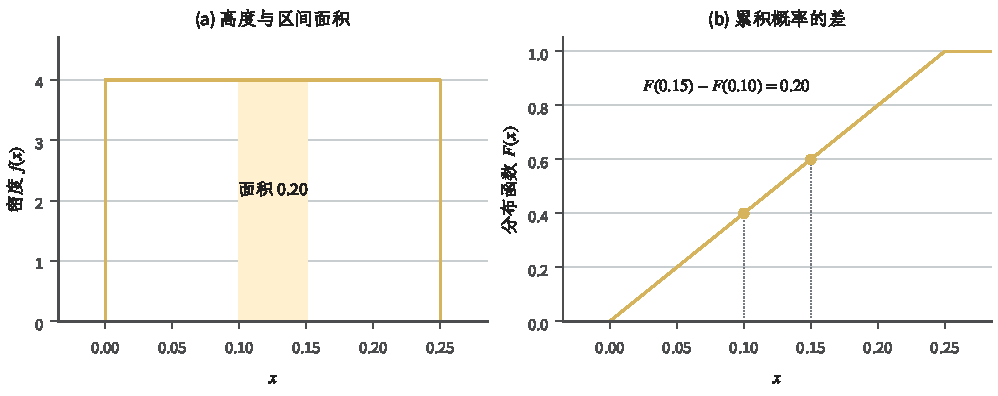
\includegraphics[width=\linewidth]{figures/math-preparation/probability-discrete/probability-density-cdf.pdf}
  \caption{区间\([0,1/4]\)上的均匀分布（解析式教学图）。左图阴影为\([0.10,0.15]\)的概率\(0.20\)，密度高度为\(4\)；右图的概率是\(F(0.15)-F(0.10)\)，两个端点本身均没有正概率质量。}
  \label{fig:probability-density-cdf}
\end{figure*}

\subsubsection{期望与分布积分}

对非负随机变量\(X\)，定义
\[ \mathbb{E}[X]
  =\int_{\Omega}X(\omega)\,\mathrm{d}\mathbb{P}(\omega). \]
对一般实随机变量，写\(X=X^+-X^-\)。当
\(\mathbb{E}[|X|]<\infty\)时，正负两部分积分都有限，此时称\(X\)可积，并定义
\(\mathbb{E}[X]=\mathbb{E}[X^+]-\mathbb{E}[X^-]\)。不要求可积便随意相减\(\infty-\infty\)没有意义。

期望只依赖\(X\)的分布。对可测函数\(g\)，只要\(g(X)\)非负或可积，就有
\begin{equation}
  \mathbb{E}[g(X)]
  =
  \int_{\mathbb{R}}g(x)\,\mathrm{d}\mathbb{P}_X(x).
  \label{eq:probability-lotus}
\end{equation}
离散时右侧是\(\sum_x g(x)p_X(x)\)，有密度时则是\(\int g(x)f_X(x)\,\mathrm{d}x\)。这条“无须先求\(g(X)\)分布”的积分公式，会反复用于矩、蒙特卡洛估计和分布变换。

式~\eqref{eq:probability-lotus}直接来自推送测度的定义。对指示函数
\(g=\mathbb{I}_B\)，等式两侧分别为
\(\mathbb{P}(X\in B)\)与\(\mathbb{P}_X(B)\)，所以相等。线性性把结论推广到非负简单函数；任取递增到非负可测\(g\)的简单函数列，再在两侧使用单调收敛定理，即得非负情形。可积实值函数则分别对\(g^+\)和\(g^-\)应用这一结论。这个证明同时说明，等式并不要求\(X\)有密度。

\begin{example}[带噪观测的平均目标]
\label{ex:probability-noisy-observation}
设未知信号为\(\theta\)，观测为
\[ Y=\theta+\varepsilon,
  \qquad\mathbb{E}[\varepsilon]=0. \]
只要\(\varepsilon\)可积，就有\(\mathbb{E}[Y]=\theta\)。这并未说明一次读数接近
\(\theta\)，也未说明多个读数的平均必然收敛；后者还需要抽样依赖关系和矩条件。概率模型先把目标写成分布下的平均，后续误差结论再回答有限观测能否逼近这个平均。
\end{example}

\subsection{绝对连续、密度与测度变换}
\label{sec:probability-radon-nikodym-change-measure}

熟悉的密度以Lebesgue测度为参照，概率质量函数以计数测度为参照。
两种写法共同的问题是：能否用一个参考测度下的权重表示另一个测度？
绝对连续排除参考测度完全看不到的正质量区域，Radon--Nikodym导数在这一前提下给出权重。
换测度随后复用同一个权重公式，而不必对每个分布重新推导积分。

\subsubsection{绝对连续与零集兼容性}

在有限集合上，两个概率表\((p_j)\)与\((q_j)\)可以逐项比较。若想用\(P\)下的样本计算\(Q\)下的平均，候选权重自然是\(q_j/p_j\)。但当\(p_j=0\)而\(q_j>0\)时，
\(P\)永远不会产生第\(j\)个结果，任何有限权重都无法补回这部分质量。

这一障碍在一般空间中由绝对连续刻画：参考测度看不到的集合，目标测度也不能给它
正质量。
\begin{definition}[测度的绝对连续]
\label{def:probability-absolute-continuity}
设\(\nu\)与\(\mu\)为同一可测空间\((\Omega,\mathcal{F})\)上的测度。若
\[ \mu(A)=0\Longrightarrow\nu(A)=0,
  \qquad\text{对所有 }A\in\mathcal{F}\text{成立}, \]
则称\(\nu\)对\(\mu\)\term{绝对连续}（absolute continuity），记作\(\nu\ll\mu\)。
\end{definition}
它只要求\(\mu\)的零集也是\(\nu\)的零集，并不表示\(\nu(A)\leq\mu(A)\)，
也不自动提供有界的密度比。

\subsubsection{有限分割上的密度表示}

先设\(\mu\)与\(\nu\)为有限测度，取有限可测分割
\(\Omega=A_1\mathbin{\dot\cup}\cdots\mathbin{\dot\cup}A_m\)，并假设\(\nu\ll\mu\)。
对\(\mu(A_j)>0\)的分块定义
\[ r(\omega)=\frac{\nu(A_j)}{\mu(A_j)},
  \qquad \omega\in A_j; \]
在\(\mu(A_j)=0\)的分块上令\(r=0\)。绝对连续性保证后一类分块也满足\(\nu(A_j)=0\)。因此，对任意由这些分块组成的事件\(A\)，
\[ \nu(A)=\int_A r\,\mathrm{d}\mu. \]
对在各分块上取有限实常数的函数\(g\)，逐项相加还给出
\begin{equation}
  \int_{\Omega}g\,\mathrm{d}\nu
  =
  \int_{\Omega}gr\,\mathrm{d}\mu.
  \label{eq:probability-finite-change-measure}
\end{equation}
一般定理要做的事，是在没有预先给定有限分块时构造同样的\(r\)
\scite{math-kallenberg2021probability}

\begin{theorem}[Radon--Nikodym定理]
\label{thm:probability-radon-nikodym}
设\(\mu\)与\(\nu\)是\((\Omega,\mathcal{F})\)上的\(\sigma\)有限测度，且
\(\nu\ll\mu\)。则存在非负可测函数\(r\)，使每个\(A\in\mathcal{F}\)都满足
\begin{equation}
  \nu(A)=\int_A r\,\mathrm{d}\mu.
  \label{eq:probability-rn-representation}
\end{equation}
函数\(r\)在\(\mu\)-几乎处处意义下唯一，记为\(r=\mathrm{d}\nu/\mathrm{d}\mu\)，称为\term{Radon--Nikodym导数}
（Radon--Nikodym derivative）。
\end{theorem}

\begin{proof}
先设\(\mu,\nu\)有限，并令\(\lambda=\mu+\nu\)。在线性空间
\(L^2(\lambda)\)上定义
\[
  T(f)=\int f\,\mathrm{d}\nu.
\]
由于\(\nu\leq\lambda\)，Cauchy--Schwarz不等式给出
\[
  |T(f)|
  \leq\int|f|\,\mathrm{d}\nu
  \leq\nu(\Omega)^{1/2}
       \left(\int f^2\,\mathrm{d}\nu\right)^{1/2}
  \leq\nu(\Omega)^{1/2}\lVert f\rVert_{L^2(\lambda)}.
\]
因此\(T\)是有界线性泛函。由第~\ref{chap:functional-analysis-and-approximation}章的Riesz表示定理，存在
\(g\in L^2(\lambda)\)，使
\[
  \int f\,\mathrm{d}\nu=\int fg\,\mathrm{d}\lambda,
  \qquad f\in L^2(\lambda).
\]
取\(f=\mathbb{I}_A\)可得\(\nu(A)=\int_Ag\,\mathrm{d}\lambda\)。若
\(A=\{g<0\}\)具有正测度，则对集合\(\{g\leq-1/k\}\)取指示函数会得到
\(\nu(\{g\leq-1/k\})<0\)的矛盾，故\(g\geq0\)几乎处处。又因为
\(\mu(A)=\lambda(A)-\nu(A)=\int_A(1-g)\,\mathrm{d}\lambda\geq0\)，同理有
\(g\leq1\)几乎处处。

令\(C=\{g=1\}\)。在\(C\)上有
\(\mu(C)=\int_C(1-g)\,\mathrm{d}\lambda=0\)，而\(\nu\ll\mu\)推出
\(\nu(C)=0\)。另一方面，\(\nu(C)=\int_Cg\,\mathrm{d}\lambda=\lambda(C)\)，所以
\(\lambda(C)=0\)。于是可以在其余部分定义
\[
  r=\frac{g}{1-g},
\]
并在\(C\)上任取值。由
\(\mathrm{d}\mu=(1-g)\,\mathrm{d}\lambda\)，对每个\(A\in\mathcal{F}\)都有
\[
  \int_A r\,\mathrm{d}\mu
  =\int_A\frac{g}{1-g}(1-g)\,\mathrm{d}\lambda
  =\int_Ag\,\mathrm{d}\lambda
  =\nu(A).
\]

若\(r_1,r_2\)都满足该表示，则对
\(A_k=\{r_1\geq r_2+1/k\}\)有
\[
  0=\int_{A_k}(r_1-r_2)\,\mathrm{d}\mu
  \geq\frac{1}{k}\mu(A_k),
\]
故\(\mu(A_k)=0\)。对\(k\)取并集得到\(r_1\leq r_2\)几乎处处；交换二者即得唯一性。

对\(\sigma\)有限的\(\mu,\nu\)，分别取有限测度覆盖并求交，可以把\(\Omega\)写成可数个互不相交、在两种测度下均有限的可测分块。在每个分块上使用上述构造，再把各块导数拼接，便得到全空间上的\(r\)。拼接后的表示可先对有限个分块验证，再由单调收敛推广到全部分块。
\end{proof}

这个证明先让\(\lambda=\mu+\nu\)同时支配两种测度，再把测度\(\nu\)表示为
\(L^2(\lambda)\)中的函数\(g\)。绝对连续性只用于排除\(g=1\)承载正质量，保证比值
\(g/(1-g)\)能够成为相对于\(\mu\)的密度。构造得到的是可测密度，并没有得到逐点上界。

\subsubsection{换测度公式与权重风险}

\begin{theorem}[换测度积分公式]
\label{thm:probability-change-measure-integral}
若\(\nu\ll\mu\)，\(r=\mathrm{d}\nu/\mathrm{d}\mu\)，则对每个非负可测函数\(g\)，
\[ \int g\,\mathrm{d}\nu
  =\int gr\,\mathrm{d}\mu. \]
只要\(g\)在\(\nu\)下可积，同一等式也对实值\(g\)成立。
\end{theorem}

\begin{proof}
对指示函数\(g=\mathbb{I}_A\)，结论就是Radon--Nikodym表示。由线性性，它对非负简单函数成立。任取非负可测\(g\)，选择简单函数\(g_n\uparrow g\)，分别在
\(\nu\)和\(\mu\)下使用单调收敛定理即可。对可积实值函数，再分别处理\(g^+\)与\(g^-\)。
\end{proof}

密度比存在、有界和具有有限二阶矩是三项不同条件。若\(P\ll Q\)，则\(w=\mathrm{d}P/\mathrm{d}Q\)存在且\(\mathbb{E}_Q[w]=1\)，但这不推出
\(\lVert w\rVert_\infty<\infty\)，也不推出\(\mathbb{E}_Q[w^2]<\infty\)。例如在\((0,1)\)上令\(Q\)为均匀分布，取
\[ w(x)=\frac{1}{2\sqrt{x}}. \]
它的积分为\(1\)，所以定义一个\(P\ll Q\)；但\(w\)无界，且\(\int_0^1w(x)^2\,\mathrm{d}x=\infty\)。换测度恒等式仍成立，使用该权重的蒙特卡洛估计却可能没有有限方差。

有限表可以直接核对权重方向。设参考分布\(Q\)在三个结果上的概率为
\((0.5,0.4,0.1)\)，目标分布\(P\)为\((0.2,0.3,0.5)\)，则
\[
  w=\frac{\mathrm{d}P}{\mathrm{d}Q}=(0.4,0.75,5).
\]
对取值\(g=(1,2,4)\)，有
\[
  \mathbb{E}_P[g]=2.8
  =0.5(0.4)(1)+0.4(0.75)(2)+0.1(5)(4)
  =\mathbb{E}_Q[wg].
\]
第三个结果在\(Q\)下少见，却在\(P\)下承载一半质量，所以产生大权重。若把参考概率
\(0.1\)改成\(0\)而保持目标概率\(0.5\)，则\(P\not\ll Q\)，任何重加权都无法从
\(Q\)样本恢复这部分目标质量。

图~\ref{fig:probability-importance-weights}显示，权重改变的是每个结果对平均的贡献，而不是把观测值\(g_j\)解释为概率。未加权平均为\(1.7\)，加权平均为\(2.8\)；第三个结果的贡献从\(0.4\)增至\(2\)，也预示它偶尔出现时会显著推动估计值。

\begin{figure*}[htbp]
  \centering
  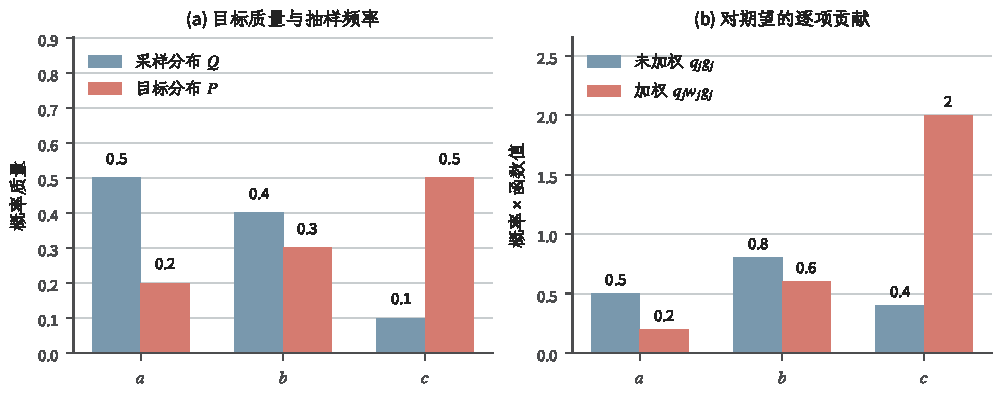
\includegraphics[width=\linewidth]{figures/math-preparation/probability-discrete/probability-importance-weights.pdf}
  \caption{三结果换测度的有限构造。左图比较采样分布\(Q\)与目标分布\(P\)，右图比较\(q_jg_j\)与\(q_jw_jg_j=p_jg_j\)。各柱从零起画；右图柱高之和分别为\(1.7\)和\(2.8\)，并非单点概率。}
  \label{fig:probability-importance-weights}
\end{figure*}

绝对连续性也决定几乎处处结论能否转移。若\(P\ll Q\)，且
\(|g|\leq M\)在\(Q\)下几乎处处成立，则违背上界的集合是\(Q\)-零集，因而也是
\(P\)-零集；同一上界在\(P\)下仍成立。反向转移需要\(Q\ll P\)，不能只凭
\(P\ll Q\)得到。若\(|g|\leq B\)，则
\[
  \mathbb{E}_Q[w^2g^2]\leq B^2\mathbb{E}_Q[w^2],
\]
所以权重二阶矩有限是有界被积函数获得有限重加权方差的充分条件。把权重截为
\(w_c=\min\{w,c\}\)会限制波动，但
\(\mathbb{E}_Q[w_cg]\)与\(\mathbb{E}_P[g]\)之差为
\(-\mathbb{E}_Q[(w-c)_+g]\)，一般不为零。

\subsection{联合、边缘与条件分布}
\label{sec:probability-joint-marginal-conditional}

换测度在同一积分对象上改变概率权重；条件化则根据已经观察到的变量重新描述未知结果。
离散条件概率可以直接相除，连续变量的单点通常没有正概率，不能沿用同一个分母解释。
概率核把“对每个条件值给一个分布”组织成可测对象，正则条件分布的存在条件由此成为必要问题。

\subsubsection{联合分布与边缘分布}

随机向量\((X,Y)\)的联合分布是映射\(\omega\mapsto(X(\omega),Y(\omega))\)在乘积空间上诱导的概率测度。离散情形中，
联合质量\(p_{X,Y}(x,y)\)给出完整表格，边缘分布由求和消去另一坐标：
\[ p_X(x)=\sum_y p_{X,Y}(x,y),
  \qquad p_Y(y)=\sum_x p_{X,Y}(x,y). \]
若联合分布有密度，则相应运算变为
\[ f_X(x)=\int f_{X,Y}(x,y)\,\mathrm{d}y. \]
一般情形不需要质量函数或密度。记坐标投影为\(\pi_X(x,y)=x\)，则边缘分布就是联合分布经\(\pi_X\)的推送：
\[
  \mathbb{P}_X(A)
  =\mathbb{P}_{(X,Y)}(A\times\mathcal{Y}).
\]
对非负可测函数\(g\)，式~\eqref{eq:probability-lotus}给出
\[
  \int g(x)\,\mathbb{P}_X(\mathrm{d}x)
  =
  \int g\bigl(\pi_X(x,y)\bigr)\,
       \mathbb{P}_{(X,Y)}(\mathrm{d}x,\mathrm{d}y).
\]
若联合分布有密度，再对右侧使用Tonelli定理，才得到对\(y\)积分的边缘密度公式。因而“边缘化”首先是测度推送，求和或积分只是它在特定参考测度下的表达。

边缘化会丢掉变量如何共同变化的信息。两个不同联合分布可以拥有完全相同的两个边缘分布。

当\(p_X(x)>0\)时，离散条件质量定义为
\[ p_{Y\mid X}(y\mid x)
  =\frac{p_{X,Y}(x,y)}{p_X(x)}. \]
因此有乘法公式
\[ p_{X,Y}(x,y)=p_X(x)p_{Y\mid X}(y\mid x). \]
若\(p_Y(y)>0\)，把联合质量按另一顺序分解便得到Bayes公式
\begin{equation}
  p_{X\mid Y}(x\mid y)
  =
  \frac{p_{Y\mid X}(y\mid x)p_X(x)}
       {\sum_{x'}p_{Y\mid X}(y\mid x')p_X(x')}.
  \label{eq:probability-discrete-bayes}
\end{equation}
分母是观测\(y\)的边缘概率，既负责归一化，也要求观测并非零概率事件。

连续密度公式是同一分解的特例。若\((X,Y)\)相对于乘积参考测度有联合密度
\(f_{X,Y}\)，且\(0<f_X(x)<\infty\)，则
\[
  f_{Y\mid X}(y\mid x)
  =\frac{f_{X,Y}(x,y)}{f_X(x)}
\]
非负并对\(y\)积分为\(1\)。它满足
\(f_{X,Y}(x,y)=f_X(x)f_{Y\mid X}(y\mid x)\)。在
\(f_X(x)=0\)或\(f_X(x)=\infty\)的点上，不能使用这个比值；这些点构成\(\mathbb P_X\)-零测集。条件核在该零测集上可统一指定一个固定概率测度，而不改变联合分布。这里选用由联合密度积分得到的边缘密度版本；任意修改过的密度版本也只能保证相应等式几乎处处成立。

\begin{example}[有限候选经过带噪观测更新]
\label{ex:probability-finite-candidate-bayes}
设信号只可能是\(\Theta\in\{-1,1\}\)，先验概率均为\(1/2\)。传感器以概率\(0.8\)报告正确符号。观测\(Y=1\)后，
\[ \mathbb{P}(\Theta=1\mid Y=1)
  =\frac{0.8\times0.5}{0.8\times0.5+0.2\times0.5}=0.8. \]
观测并未把候选集合改成一个确定点，而是改变了两个候选的相对权重。若某个观测在所有
候选下概率都为零，公式分母为零，条件分布不能靠这个比值定义。
\end{example}

\subsubsection{概率核与条件化的可测性}

当条件变量连续时，事件\(\{X=x\}\)常有零概率，直接相除不再可行。需要把“每个条件值对应一个分布”组织成能继续积分的对象。
\begin{definition}[概率核]
  \label{def:probability-kernel}
  给定可测空间\((\mathcal X,\mathcal A)\)、\((\mathcal Y,\mathcal B)\)，\term{概率核}（probability kernel）是映射
  \[ K:\mathcal X\times\mathcal B\to[0,1], \]
  满足：对每个\(x\in\mathcal X\)，\(K(x,\cdot)\)是\((\mathcal Y,\mathcal B)\)上的概率测度；对每个\(B\in\mathcal B\)，\(x\mapsto K(x,B)\)是\(\mathcal A\)-可测函数。
\end{definition}
第一项保证每个条件值给出合法分布，
第二项保证再对\(X\)积分是合法运算。

可测并不等于连续。例如取\(X\sim\mathcal N(0,1)\)、\(Y=\mathbb I\{X\geq0\}\)，则\(K(x,\{1\})=\mathbb I\{x\geq0\}\)是合法概率核在事件\(\{1\}\)上的取值，却在\(x=0\)处跳变。条件值\(x\)可以连续取值，条件分布随\(x\)变化仍可不连续。

\begin{definition}[正则条件分布]
  \label{def:probability-regular-conditional-distribution}
若概率核\(K\)对所有\(A\in\mathcal A\)、\(B\in\mathcal B\)满足
\begin{equation}
  \mathbb{P}(X\in A,Y\in B)
  =
  \int_A K(x,B)\,\mathbb{P}_X(\mathrm{d}x),
  \label{eq:probability-regular-conditional-kernel}
\end{equation}
就把\(K(x,\cdot)\)称为\(Y\)给定\(X=x\)的一个\term{正则条件分布}（regular conditional distribution）。
\end{definition}
对每个固定可测集\(B\)，两个版本的\(K(x,B)\)在\(\mathbb P_X\)-几乎处处意义下相同；若\(\mathcal Y\)是下面的标准Borel空间，还可选取一个共同零测集，使其外的条件概率测度相同。零概率条件点上的取值通常不能由联合分布唯一决定。

\subsubsection{正则条件分布的存在条件}

逐个条件事件的概率能够定义，并不保证它们能拼成一个共同的概率核。下面的可测空间条件为这种拼接提供保证。
\begin{definition}[Polish空间]
  \label{def:probability-polish-space}
拓扑空间若存在一个诱导该拓扑的完备、可分度量，就称为Polish空间。可分表示含有可数稠密子集；完备性表示该度量下每个Cauchy序列都收敛到空间中的点。
\end{definition}
欧氏空间就是一个例子。这里既需要能用可数对象逼近，也需要极限仍落在所研究的空间内；标准Borel空间只保留这种空间的可测结构。
\begin{definition}[标准Borel空间]
  \label{def:probability-standard-borel-space}
  可测空间称为\term{标准Borel空间}（standard Borel space），若它与某个完备可分度量空间的Borel子集可测同构，即存在双射，且该双射及其逆映射都可测。
\end{definition}
“可分”表示度量空间含有可数稠密子集。若\(X\)与\(Y\)的状态空间都是标准Borel空间，则上述正则条件分布存在。实数空间、欧氏空间、可数集合以及配备适当Borel结构的常见可分函数空间都属于这一范围。

这一存在结论依赖可数生成结构与条件期望。下一小节定义条件期望以后，再说明逐个事件上的条件平均如何组成同一个概率核。

在完全一般的可测空间上，正则条件分布可能不存在。此时条件期望仍可相对于子\(\sigma\)代数定义，但不能未经说明就把它写成每个点\(x\)上的条件密度。后续模型
通常工作在标准Borel空间中；使用\(p(y\mid x)\)时，应同时确认密度所依赖的参考测度及其适用的几乎处处范围。

\subsection{期望、方差与条件期望}
\label{sec:probability-expectation-conditional-expectation}

\subsubsection{均值、方差与协方差}

可积随机变量的均值记作\(\mu_X=\mathbb{E}[X]\)。若\(\mathbb{E}[X^2]<\infty\)，其方差为
\[ \operatorname{Var}(X)
  =\mathbb{E}\bigl[(X-\mu_X)^2\bigr]=\mathbb{E}[X^2]-\mu_X^2. \]
对二阶可积的\(X,Y\)，协方差为
\[ \operatorname{Cov}(X,Y)
  =\mathbb{E}\bigl[(X-\mathbb{E}X)(Y-\mathbb{E}Y)\bigr]. \]
Cauchy--Schwarz不等式保证它有限。方差满足
\[ \operatorname{Var}(aX+b)=a^2\operatorname{Var}(X), \]
而
\[ \operatorname{Var}(X+Y)
  =\operatorname{Var}(X)+\operatorname{Var}(Y)+2\operatorname{Cov}(X,Y). \]
只有协方差为零时，方差才直接相加；独立是协方差为零的充分条件，但通常不是必要条件。

\subsubsection{条件期望与信息约束}

子\(\sigma\)代数\(\mathcal{G}\subseteq\mathcal{F}\)表示当前可用信息。预测值必须只使用这些信息，又应在每个可识别的分组内保持平均值。
\begin{definition}[观测生成的信息]
  \label{def:probability-generated-information}
若\(X:\Omega\to(\mathcal X,\mathcal A)\)是随机变量，记
\(\sigma(X)=\{X^{-1}(A):A\in\mathcal A\}\)。它是使\(X\)可测的最小\(\sigma\)代数，表示仅观察\(X\)能够区分的事件。多个观测生成的信息是包含它们全部可测逆像的最小\(\sigma\)代数。
\end{definition}
例如只观察分组编号，就不能在同一组内区分两个原始结果。写\(\mathbb E[Y\mid X]\)时，真正限制答案的信息是\(\sigma(X)\)，不是单个零概率事件\(\{X=x\}\)。
\begin{definition}[条件期望]
  \label{def:probability-conditional-expectation}
对\(X\in L^1(\mathbb P)\)，\term{条件期望}（conditional expectation）
\(\mathbb{E}[X\mid\mathcal{G}]\)是满足下列两项条件的可积随机变量\(Z\)：
\[ Z\text{ 对 }\mathcal{G}\text{ 可测},
  \qquad\int_A Z\,\mathrm{d}\mathbb{P}=\int_A X\,\mathrm{d}\mathbb{P}\quad(A\in\mathcal{G}). \]
\end{definition}
第一项要求答案只能使用\(\mathcal{G}\)中的信息，第二项要求它在每个可由当前信息识别的事件上保留\(X\)的平均
\scite{math-kallenberg2021probability}

\begin{theorem}[条件期望的存在与唯一性]
\label{thm:probability-conditional-expectation-existence}
若\(X\in L^1(\mathbb{P})\)，则\(\mathbb{E}[X\mid\mathcal{G}]\)存在，并在几乎处处意义下唯一。
\end{theorem}

\begin{proof}
先设\(X\geq0\)。在\((\Omega,\mathcal{G})\)上定义有限测度
\[ \nu(A)=\int_A X\,\mathrm{d}\mathbb{P}. \]
若\(\mathbb{P}(A)=0\)，则\(\nu(A)=0\)，所以\(\nu\ll\mathbb{P}|_{\mathcal{G}}\)。Radon--Nikodym定理给出非负、
\(\mathcal{G}\)-可测的\(Z\)，使\(\nu(A)=\int_A Z\,\mathrm{d}\mathbb{P}\)。对一般可积\(X\)，分别对
\(X^+\)与\(X^-\)使用这一构造并取差，即得存在性。

若\(Z_1,Z_2\)都满足定义，令\(D=Z_1-Z_2\)。对每个\(A\in\mathcal{G}\)，\(\int_A D\,\mathrm{d}\mathbb{P}=0\)。若
\(\mathbb{P}(D>0)>0\)，则某个集合\(A_k=\{D\geq1/k\}\)具有正概率，从而
\[ \int_{A_k}D\,\mathrm{d}\mathbb{P}
  \geq\frac{1}{k}\mathbb{P}(A_k)>0, \]
产生矛盾。因此\(D\leq0\)几乎处处。交换\(Z_1,Z_2\)可得\(D\geq0\)几乎处处，故二者几乎处处相等。
\end{proof}

若\(X\)本来就对\(\mathcal{G}\)可测，则\(\mathbb{E}[X\mid\mathcal{G}]=X\)几乎处处。若\(X\)与\(\mathcal{G}\)
独立，则条件期望等于常数\(\mathbb{E}[X]\)。若\(U\)有界且\(\mathcal{G}\)-可测，则
\begin{equation}
  \mathbb{E}[UX\mid\mathcal{G}]
  =
  U\mathbb{E}[X\mid\mathcal{G}].
  \label{eq:probability-taking-out-known-factor}
\end{equation}
可积的非有界\(U\)需要另外核对乘积可积性，不能仅凭“已知量可提出”略去条件。

有限分组把抽象定义化成逐组平均。若
\(A_1,\ldots,A_m\)是有限可测分割，
\(\mathcal{G}=\sigma(A_1,\ldots,A_m)\)，且每个
\(\mathbb{P}(A_j)>0\)，则
\begin{equation}
  \mathbb{E}[X\mid\mathcal{G}]
  =
  \sum_{j=1}^{m}
  \frac{\mathbb{E}[X\mathbb{I}_{A_j}]}
       {\mathbb{P}(A_j)}
  \mathbb{I}_{A_j}.
  \label{eq:probability-finite-partition-conditional-expectation}
\end{equation}
若某个分组概率为零，该组上的取值可以任意指定，因为条件期望只在几乎处处意义下唯一。

表~\ref{tab:probability-finite-partition-predictions}给出一个可复核例子。令
\(\mathcal{G}\)只能区分
\(A=\{\omega_1,\omega_2\}\)与
\(B=\{\omega_3,\omega_4\}\)。不使用分组信息时，最佳常数预测是
\(U_0=\mathbb{E}X=3.4\)；规则\(U_{\mathrm{grp}}\)虽然按组取值，却随意地在
\(A,B\)上分别预测\(0,4\)；条件均值\(m=\mathbb{E}[X\mid\mathcal{G}]\)则在两组
上分别等于\(1.2,5.6\)。
\begin{table}[htbp]
  \centering
  \small
  \begin{tabular}{ccccccc}
    \toprule
    结果 & 概率 & \(X\) & 分组 & \(U_0\) & \(U_{\mathrm{grp}}\) & \(m\) \\
    \midrule
    \(\omega_1\) & \(0.2\) & \(0\) & \(A\) & \(3.4\) & \(0\) & \(1.2\) \\
    \(\omega_2\) & \(0.3\) & \(2\) & \(A\) & \(3.4\) & \(0\) & \(1.2\) \\
    \(\omega_3\) & \(0.1\) & \(4\) & \(B\) & \(3.4\) & \(4\) & \(5.6\) \\
    \(\omega_4\) & \(0.4\) & \(6\) & \(B\) & \(3.4\) & \(4\) & \(5.6\) \\
    \midrule
    \multicolumn{4}{r}{平方风险\(\ \mathbb{E}[(X-U)^2]\)} &
    \(5.64\) & \(2.80\) & \(0.80\) \\
    \bottomrule
  \end{tabular}
  \caption{有限分组下的三类预测。分组信息使预测可以随\(A,B\)变化，但只有逐组条件
  均值在全部\(\mathcal{G}\)-可测平方可积预测中达到最小平方风险。}
  \label{tab:probability-finite-partition-predictions}
\end{table}
三列风险依次说明不同问题：获得分组信息可以优于无信息常数，但使用信息本身不保证已经
最优；式~\eqref{eq:probability-finite-partition-conditional-expectation}还要在每组
内选择正确的条件平均。

构造思路可以从可数生成族看清。先在\(\mathcal{Y}\)的一个可数、能区分概率测度的集合族上，对每个\(B\)构造
\(\mathbb{P}(Y\in B\mid\sigma(X))\)；再选取这些条件期望关于\(X\)的可测版本。在去掉一个共同零测集后，这些数值满足有限可加性和连续性，扩张定理把它们唯一延拓为
\(\mathcal{Y}\)上的概率测度。标准Borel结构提供的可数性和可分性，正是把逐个事件的版本整理成同一个概率核所需的条件。

\subsubsection{塔式性质与全期望}

\begin{theorem}[塔式性质]
\label{thm:probability-tower-property}
若\(X\in L^1\)，且\(\mathcal{H}\subseteq\mathcal{G}\subseteq\mathcal{F}\)，则
\[ \mathbb{E}\bigl[\mathbb{E}[X\mid\mathcal{G}]
  \mid\mathcal{H}\bigr]=\mathbb{E}[X\mid\mathcal{H}] \]
几乎处处成立。
\end{theorem}

\begin{proof}
左侧对\(\mathcal{H}\)可测。对任意\(A\in\mathcal{H}\)，由于\(A\in\mathcal{G}\)，条件期望定义给出
\[
  \int_A
  \mathbb{E}\bigl[\mathbb{E}[X\mid\mathcal{G}]
  \mid\mathcal{H}\bigr]\,\mathrm{d}\mathbb{P}
  =
  \int_A\mathbb{E}[X\mid\mathcal{G}]\,\mathrm{d}\mathbb{P}
  =
  \int_A X\,\mathrm{d}\mathbb{P}.
\]
左侧因而满足\(X\)关于\(\mathcal{H}\)的条件期望定义，唯一性给出结论。
\end{proof}

取\(\mathcal{H}=\{\varnothing,\Omega\}\)，便得到\term{全期望公式}（law of total expectation）
\begin{equation}
  \mathbb{E}\bigl[\mathbb{E}[X\mid\mathcal{G}]\bigr]
  =
  \mathbb{E}[X].
  \label{eq:probability-total-expectation}
\end{equation}
这说明条件化改变可用信息，却不改变再平均后的总体均值。

\subsubsection{全方差分解}

设\(X\in L^2\)，记\(m=\mathbb{E}[X\mid\mathcal{G}]\)。分解
\[ X-\mathbb{E}X=(X-m)+(m-\mathbb{E}X). \]
在展开平方前，需要先确认条件均值仍然二阶可积。对凸函数\(u\mapsto u^2\)使用条件
Jensen不等式，有
\[
  |m|^2
  \leq
  \mathbb{E}[X^2\mid\mathcal{G}].
\]
再取期望并使用全期望公式，得到
\[
  \mathbb{E}[m^2]\leq\mathbb{E}[X^2]<\infty.
\]
因此\(m\in L^2\)，上面分解中的两项都二阶可积，其乘积由Cauchy--Schwarz不等式保证可积。又因为第二项对
\(\mathcal{G}\)可测，而\(\mathbb{E}[X-m\mid\mathcal{G}]=0\)，所以交叉项期望为
\[ \mathbb{E}\bigl[(X-m)(m-\mathbb{E}X)\bigr]
  =\mathbb{E}\left[(m-\mathbb{E}X)\mathbb{E}[X-m\mid\mathcal{G}]\right]=0. \]
展开平方得到\term{全方差公式}（law of total variance）
\begin{equation}
  \operatorname{Var}(X)
  =
  \mathbb{E}\bigl[\operatorname{Var}(X\mid\mathcal{G})\bigr]
  +
  \operatorname{Var}\bigl(\mathbb{E}[X\mid\mathcal{G}]\bigr),
  \label{eq:probability-total-variance}
\end{equation}
其中
\[ \operatorname{Var}(X\mid\mathcal{G})
  =\mathbb{E}\bigl[(X-m)^2\mid\mathcal{G}\bigr]. \]
第一项是获得\(\mathcal{G}\)后仍无法解释的平均波动，第二项是不同信息状态之间的可解释波动。

\subsubsection{条件期望的平方损失最优性}

\begin{theorem}[条件均值的平方损失最优性]
\label{thm:probability-conditional-mean-l2-projection}
设\(X\in L^2(\mathbb{P})\)。在所有\(\mathcal{G}\)-可测且二阶可积的随机变量\(U\)中，
\[ m=\mathbb{E}[X\mid\mathcal{G}] \]
唯一地在几乎处处意义下最小化\(\mathbb{E}[(X-U)^2]\)。
\end{theorem}

\begin{proof}
\(L^2(\mathcal{G})\)是\(L^2(\mathcal{F})\)的闭线性子空间，上文的条件Jensen不等式已经说明
\(m\in L^2(\mathcal{G})\)。对每个\(U\in L^2(\mathcal{G})\)，Cauchy--Schwarz不等式保证
\((X-m)U\)可积，因而可以提出已知因子并使用塔式性质，得到
\[ \mathbb{E}[(X-m)U]
  =\mathbb{E}\left[U\mathbb{E}[X-m\mid\mathcal{G}]\right]=0. \]
所以\(X-m\)与整个\(L^2(\mathcal{G})\)正交。定理~\ref{thm:functional-hilbert-projection}说明\(m\)是\(X\)到该闭子空间的正交投影。也可直接展开
\begin{equation}
  \mathbb{E}[(X-U)^2]
  =
  \mathbb{E}[(X-m)^2]
  +
  \mathbb{E}[(m-U)^2],
  \label{eq:probability-pythagorean-prediction}
\end{equation}
交叉项因正交性消失。第二项非负，且仅当\(U=m\)几乎处处时为零。
\end{proof}

条件期望的存在只需要\(X\in L^1\)，这时它由Radon--Nikodym导数给出。“正交投影”和平方损失最优性则需要\(X\in L^2\)。若二阶矩无限，条件期望仍可能
存在，但不能使用Hilbert空间几何或有限平方风险。

\subsubsection{条件换测度}

设\(Q\ll P\)，并记\(L=\mathrm{d}Q/\mathrm{d}P\)。对\(X\in L^1(Q)\)，在\(\mathbb{E}_P[L\mid\mathcal{G}]>0\)处有
\begin{equation}
  \mathbb{E}_Q[X\mid\mathcal{G}]
  =
  \frac{\mathbb{E}_P[LX\mid\mathcal{G}]}
       {\mathbb{E}_P[L\mid\mathcal{G}]}.
  \label{eq:probability-conditional-change-measure}
\end{equation}
为验证这个候选变量确实是条件期望，记
\[
  D=\mathbb{E}_P[L\mid\mathcal{G}],
  \qquad
  N=\mathbb{E}_P[LX\mid\mathcal{G}],
\]
并在\(\{D>0\}\)上令\(Z=N/D\)，在\(\{D=0\}\)上令\(Z=0\)。分母零集在\(Q\)下可以忽略，因为
\[
  Q(D=0)
  =
  \mathbb{E}_P[L\mathbb{I}\{D=0\}]
  =
  \mathbb{E}_P[D\mathbb{I}\{D=0\}]
  =0.
\]
条件期望的单调性还给出
\[
  |N|
  \leq
  \mathbb{E}_P[L|X|\mid\mathcal{G}].
\]
在\(\{D=0\}\)上，非负变量\(L\mathbb{I}\{D=0\}\)的期望为零，因而\(L=0\)几乎处处。于是
\[
  \mathbb{E}_P\left[
    \mathbb{E}_P[L|X|\mid\mathcal{G}]
    \mathbb{I}\{D=0\}
  \right]
  =
  \mathbb{E}_P[L|X|\mathbb{I}\{D=0\}]
  =0,
\]
上面的条件三角不等式进而说明\(N=0\)在\(\{D=0\}\)上几乎处处成立。因此\(DZ=N\)几乎处处，而且
\[
  \begin{aligned}
    \mathbb{E}_Q|Z|
    &=
    \mathbb{E}_P[L|Z|]
    =
    \mathbb{E}_P[D|Z|]\\
    &=
    \mathbb{E}_P\bigl[|N|\mathbb{I}\{D>0\}\bigr]
    \leq
    \mathbb{E}_P[L|X|]
    =
    \mathbb{E}_Q|X|<\infty.
  \end{aligned}
\]
这里把\(\mathcal{G}\)-可测的非负因子\(|Z|\)提出条件期望，可以由有界截断和单调收敛得到。候选变量的可积性建立后，对
\(A\in\mathcal{G}\)可合法地计算
\[
  \begin{aligned}
    \int_A Z\,\mathrm{d}Q
    &=
    \int_A ZL\,\mathrm{d}P
    =
    \int_A Z\mathbb{E}_P[L\mid\mathcal{G}]\,\mathrm{d}P\\
    &=
    \int_A \mathbb{E}_P[LX\mid\mathcal{G}]\,\mathrm{d}P
    =
    \int_A LX\,\mathrm{d}P
    =
    \int_A X\,\mathrm{d}Q.
  \end{aligned}
\]
因此\(Z\)满足\(X\)在\(Q\)下关于\(\mathcal{G}\)的条件期望定义。公式\eqref{eq:probability-conditional-change-measure}是Bayes更新的一般测度形式；
分母零集与候选变量可积性都需要像上面这样核对。

用有限分组可以看出分母为何不可省略。设参考分布\(P\)把四个结果
\(\omega_1,\ldots,\omega_4\)分别赋予概率\((0.4,0.1,0.1,0.4)\)，目标分布
\(Q\)赋予\((0.1,0.4,0.2,0.3)\)。令信息\(\mathcal{G}\)只区分
\(A=\{\omega_1,\omega_2\}\)和\(A^{\mathsf c}\)，并令
\(X=(0,1,0,1)\)。权重\(L\)在四点上的值为\((0.25,4,2,0.75)\)。在\(A\)内，
\[
  \mathbb{E}_P[LX\mid\mathcal{G}]
  =\frac{0.4}{0.5}=0.8,\qquad
  \mathbb{E}_P[L\mid\mathcal{G}]
  =\frac{0.1+0.4}{0.5}=1,
\]
所以目标条件均值为\(0.8\)，与
\(\mathbb{E}_Q[X\mid A]=0.4/(0.1+0.4)\)一致。直接用某个无条件权重乘
\(\mathbb{E}_P[X\mid A]=0.2\)不会得到目标条件均值；条件化后必须在每个信息分组内重新归一化。

\subsection{独立与条件独立}
\label{sec:probability-moments-independence}

\subsubsection{独立、不相关与非线性依赖}

若随机变量\(X,Y\)满足
\[ \mathbb{P}(X\in A,Y\in B)
  =\mathbb{P}(X\in A)\mathbb{P}(Y\in B) \]
对所有Borel集合\(A,B\)成立，就称二者\term{独立}（independent）。独立意味着所有可积可分函数都满足
\(\mathbb{E}[g(X)h(Y)]=\mathbb{E}[g(X)]\mathbb{E}[h(Y)]\)。
证明从指示函数开始：独立性正好说明结论对
\(g=\mathbb{I}_A\)、\(h=\mathbb{I}_B\)成立。线性性把它推广到简单函数，随后分别用单调收敛处理非负函数，再分解正负部分处理乘积可积的实值函数。这里必须要求相关积分有定义，不能把两个发散期望形式相乘。

协方差只检查中心化变量的一次乘积。令\(X\)在\([-1,1]\)上均匀分布，并取\(Y=X^2\)。对称性给出
\[ \operatorname{Cov}(X,Y)
  =\mathbb{E}[X^3]-\mathbb{E}[X]\mathbb{E}[X^2]=0, \]
但\(Y\)由\(X\)完全决定；知道\(X\)便能确定\(Y\)，所以二者不独立。零协方差只排除了线性二阶关联。

\subsubsection{条件独立及其运算规则}

\begin{definition}[条件独立]
  \label{def:probability-conditional-independence}
  给定随机变量\(X,Y,Z\)，若对\(X,Y\)取值空间中的所有可测集合\(A,B\)，
\[ \mathbb{P}(X\in A,Y\in B\mid Z)
  =\mathbb{P}(X\in A\mid Z)\mathbb{P}(Y\in B\mid Z) \]
几乎处处成立，就称\(X\)与\(Y\)在给定\(Z\)时条件独立，记作
\(X\perp Y\mid Z\)。
\end{definition}
它表示\(Z\)已知以后，\(X\)不再提供关于\(Y\)的额外分布信息；这不意味着去掉\(Z\)后仍独立。

条件独立满足以下常用规则：
\[
\begin{aligned}
  X\perp Y\mid Z
  &\Longrightarrow Y\perp X\mid Z
  &&\text{（对称性）},\\
  X\perp(Y,W)\mid Z
  &\Longrightarrow X\perp Y\mid Z
  &&\text{（分解）},\\
  X\perp(Y,W)\mid Z
  &\Longrightarrow X\perp Y\mid Z,W
  &&\text{（弱并）},\\
  X\perp Y\mid Z,\quad X\perp W\mid Y,Z
  &\Longrightarrow X\perp(Y,W)\mid Z
  &&\text{（收缩）}.
\end{aligned}
\]
这些规则可由条件核的乘积分解逐项验证。交性质
\[ X\perp Y\mid Z,W,\quad
  X\perp W\mid Z,Y\Longrightarrow X\perp(Y,W)\mid Z \]
并非无条件成立；严格为正的有限离散联合质量是一个常用充分条件。若分布把质量集中在
低维约束上，零概率组合会阻断所需的消元步骤。

\begin{lemma}[严格正离散分布的交性质]
  \label{lem:probability-positive-intersection}
  设$I$为有限索引集，每个$i\in I$对应取值于有限非空状态空间$\mathcal{X}_i$的随机变量$X_i$。令$p$为$\bm{X}=(X_i)_{i\in I}$在乘积状态空间$\mathcal{X}=\prod_{i\in I}\mathcal{X}_i$上的联合质量函数，且$p(\bm{x})>0$对所有$\bm{x}\in\mathcal{X}$成立。对两两不交的索引集$A,B,C,D\subseteq I$，若
  \[
    \bm{X}_A\perp\bm{X}_B\mid(\bm{X}_C,\bm{X}_D),
    \qquad
    \bm{X}_A\perp\bm{X}_D\mid(\bm{X}_C,\bm{X}_B),
  \]
  则
  \[
    \bm{X}_A\perp(\bm{X}_B,\bm{X}_D)\mid\bm{X}_C.
  \]
\end{lemma}

\begin{proof}
严格正性保证以下每个条件概率都有定义。对任意取值$\bm{a},\bm{b},\bm{c},\bm{d}$，两个前提分别给出
\[
  p(\bm{a}\mid\bm{b},\bm{c},\bm{d})
  =p(\bm{a}\mid\bm{c},\bm{d}),
  \qquad
  p(\bm{a}\mid\bm{b},\bm{c},\bm{d})
  =p(\bm{a}\mid\bm{b},\bm{c}).
\]
因此$p(\bm{a}\mid\bm{c},\bm{d})=p(\bm{a}\mid\bm{b},\bm{c})$对每个$\bm{b},\bm{d}$成立。固定任意基准值$\bm{b}^{\circ}$，右侧等于$q(\bm{a},\bm{c})=p(\bm{a}\mid\bm{b}^{\circ},\bm{c})$，不再依赖$\bm{b}$或$\bm{d}$。对$(\bm{b},\bm{d})$关于$p(\bm{b},\bm{d}\mid\bm{c})$求和可得$q(\bm{a},\bm{c})=p(\bm{a}\mid\bm{c})$，故$p(\bm{a}\mid\bm{b},\bm{c},\bm{d})=p(\bm{a}\mid\bm{c})$，这正是所需的条件独立性。
\end{proof}
严格正性使上面证明能在固定\(\bm c\)后独立改变\(\bm b\)和\(\bm d\)。若只支持部分组合，这一步会失败。一个反例是\(X=Y=W=B\)，其中\(B\)为非退化Bernoulli变量，\(Z\)取常数。给定\(W\)后\(X,Y\)都确定，所以\(X\perp Y\mid W\)；给定\(Y\)后也有\(X\perp W\mid Y\)。但\(X\)与\((Y,W)\)显然不独立，因为后者直接给出\(X\)。两个条件独立前提因而不能在这类带零概率配置的分布上推出交性质。

以分解和收缩为例可以看清这些规则使用了什么。若
\(X\perp(Y,W)\mid Z\)，则对任意可测集合\(A,B,C\)，条件核满足
\[
  K_{X,Y,W\mid Z}(A,B,C\mid z)
  =K_{X\mid Z}(A\mid z)K_{Y,W\mid Z}(B,C\mid z).
\]
令\(C\)取全集便得到
\(K_{X,Y\mid Z}=K_{X\mid Z}K_{Y\mid Z}\)，这就是分解规则。对收缩规则，假设
\[
  K_{X,Y\mid Z}=K_{X\mid Z}K_{Y\mid Z},
  \qquad
  K_{X,W\mid Y,Z}=K_{X\mid Y,Z}K_{W\mid Y,Z}.
\]
第一个条件还给出
\(K_{X\mid Y,Z}=K_{X\mid Z}\)的一个版本。沿条件乘法公式相乘可得
\[
  K_{X,Y,W\mid Z}
  =K_{X\mid Z}K_{Y\mid Z}K_{W\mid Y,Z}
  =K_{X\mid Z}K_{Y,W\mid Z},
\]
即\(X\perp(Y,W)\mid Z\)。所有等式都按相应条件变量分布的几乎处处意义理解。概率图模型部分会在这些概率规则之上另加图分离语义；图上没有边本身并不是这里定义的条件独立证明。

多元高斯分布是一个特殊情形：联合高斯随机向量的两个子向量若协方差为零，则它们独立；条件高斯中的条件协方差为零也对应条件独立。这个结论依赖高斯
密度由一、二阶矩完全确定，不能推广到一般分布。

\section{分布族与随机变换}
\label{sec:probability-families-transformations}

共同的概率对象确定后，本节给出可计算的具体分布，并研究组合变量与改变坐标后的分布。
常用分布提供建模部件，线性变换、条件化和混合说明这些部件怎样组成联合模型。
计算结果时仍要返回上一节核对参考测度、支持与条件化对象。

\subsection{用矩与变换函数描述分布}
\label{sec:probability-moment-transforms}

均值和方差便于计算，却不足以区分许多分布。若关心偏斜、尾部或独立和的分布变化，需要在这两个摘要之外保留信息：高阶矩增加摘要阶数，生成函数则把一系列摘要组织到一个函数中。

若\(\mathbb{E}[|X|^k]<\infty\)，则\(\mathbb{E}[X^k]\)称为\(k\)阶原点矩，
\(\mathbb{E}[(X-\mathbb{E}X)^k]\)称为\(k\)阶中心矩。三阶中心矩反映不对称性，四阶中心矩反映尾部与峰度，但有限低阶矩通常不能唯一确定分布。

\begin{definition}[矩母函数与累积量生成函数]
  \label{def:probability-moment-generating-functions}
设\(X\)为实随机变量。若存在\(\delta>0\)，使\(\mathbb E e^{tX}<\infty\)对全部\(|t|<\delta\)成立，则在该邻域上定义\term{矩母函数}（moment-generating function, MGF）为
\[ M_X(t)=\mathbb{E}[e^{tX}]. \]
\term{累积量生成函数}（cumulant-generating function）是
\[ K_X(t)=\log M_X(t). \]
\end{definition}
若可在积分号下求导，则\(M_X^{(k)}(0)=\mathbb{E}[X^k]\)。矩存在不保证矩母函数在原点邻域有限；例如对数正态分布拥有所有正整数阶矩，却对每个\(t>0\)都有
\(\mathbb E e^{tX}=\infty\)，因而不满足上述邻域条件。
累积量生成函数的前两阶导数分别给出均值和方差。对随机向量\(\bm{X}\)，
\[ K_{\bm{X}}(\bm{t})
  =\log\mathbb{E}\bigl[e^{\bm{t}^{\top}\bm{X}}\bigr], \]
混合偏导数给出联合累积量。独立分量使\(K_{\bm{X}}\)按坐标相加，因此所有跨分量
联合累积量为零。在矩母函数存在的适当邻域内，反向也可通过解析性得到。独立成分分析利用三阶、四阶等非高斯统计量识别协方差白化后仍隐藏的依赖；纯高斯变量
的三阶以上累积量为零，不能靠这一路径区分旋转方向。

前两阶关系可以直接核对。若存在\(\delta>0\)使
\(\mathbb{E}e^{tX}<\infty\)对\(|t|<\delta\)成立，则对更小邻域中的\(t\)，
\(|X|e^{tX}\)与\(X^2e^{tX}\)可由邻域端点的指数函数控制。第~\ref{chap:mathematical-analysis}章的积分下求导条件于是给出
\[
  M_X'(t)=\mathbb{E}[Xe^{tX}],\qquad
  M_X''(t)=\mathbb{E}[X^2e^{tX}].
\]
因为\(M_X(0)=1\)，
\[
  K_X'(0)=\frac{M_X'(0)}{M_X(0)}=\mathbb{E}X,
  \qquad
  K_X''(0)
  =M_X''(0)-M_X'(0)^2
  =\operatorname{Var}(X).
\]
独立变量\(X,Y\)满足
\(M_{X+Y}(t)=M_X(t)M_Y(t)\)，故
\(K_{X+Y}=K_X+K_Y\)；累积量可加来自独立性，而不是仅来自零协方差。

矩母函数能生成矩，也能提供尾界，但它可能在零点的任何双侧邻域都不有限。研究分布极限时，需要一个对所有实参数都存在的变换。
\begin{definition}[特征函数]
  \label{def:probability-characteristic-function}
实随机变量\(X\)的特征函数为\(\varphi_X(t)=\mathbb E e^{\mathrm i tX}\)，其中\(t\in\mathbb R\)。随机向量的版本为\(\varphi_{\bm X}(\bm t)=\mathbb E e^{\mathrm i\bm t^\top\bm X}\)。复数期望分别对实部与虚部积分。
\end{definition}
由于复指数的绝对值恒为\(1\)，特征函数总存在。它用振荡而非指数放大取值，因此与可能发散的矩母函数承担不同职责；后面将用它把独立和的分布极限转成函数的逐点极限。

\subsection{常用分布与分布族}
\label{sec:probability-common-distributions}

\subsubsection{计数、类别与等待时间}

\term{Bernoulli分布}以参数\(p\in[0,1]\)描述一次二元结果：
\[ \mathbb{P}(X=x)=p^x(1-p)^{1-x},
  \qquad x\in\{0,1\}, \]
且\(\mathbb{E}X=p\)、\(\operatorname{Var}(X)=p(1-p)\)。\(n\)个独立同分布的
Bernoulli变量之和服从\term{二项分布}
\[ \mathbb{P}(S=k)
  =\binom{n}{k}p^k(1-p)^{n-k},\qquad k=0,\ldots,n, \]
其均值和方差分别为\(np\)与\(np(1-p)\)。

若一次试验有\(K\)个类别，概率向量\(\bm{p}\)满足\(p_k\geq0\)及\(\sum_kp_k=1\)。\(n\)次独立试验的类别计数\(\bm{N}\)服从\term{多项分布}，质量为
\[ \mathbb{P}(\bm{N}=\bm{n})
  =\frac{n!}{\prod_{k=1}^{K}n_k!}\prod_{k=1}^{K}p_k^{n_k},\qquad\sum_{k=1}^{K}n_k=n. \]
其均值为\(\mathbb{E}N_k=np_k\)，协方差为\(\operatorname{Cov}(N_j,N_k)=n(p_j\mathbb{I}\{j=k\}-p_jp_k)\)。

\term{Poisson分布}以\(\lambda>0\)描述固定窗口中的稀疏计数：
\[ \mathbb{P}(N=k)
  =e^{-\lambda}\frac{\lambda^k}{k!},\qquad k=0,1,\ldots, \]
且均值、方差都为\(\lambda\)。若独立计数
\(N_j\sim\operatorname{Poisson}(\lambda_j)\)，则\(\sum_jN_j\sim\operatorname{Poisson}(\sum_j\lambda_j)\)。

\term{指数分布}以速率\(\lambda>0\)描述等待时间：
\[ f_T(t)=\lambda e^{-\lambda t}\mathbb{I}\{t\geq0\}. \]
它的均值为\(1/\lambda\)，方差为\(1/\lambda^2\)，并具有无记忆性
\[ \mathbb{P}(T>s+t\mid T>s)=\mathbb{P}(T>t). \]
无记忆性只适用于已经等待的时长不改变剩余等待分布，不表示不同等待时间自动独立。
Poisson计数与指数等待描述的是同一个齐次到达机制的两个侧面。若速率为\(\lambda\)的
Poisson过程中，\(N(t)\)记录长度为\(t\)的时间窗内的到达数，\(T_1\)是首次到达时间，
则
\[
  \mathbb{P}(T_1>t)
  =
  \mathbb{P}(N(t)=0)
  =
  e^{-\lambda t}.
\]
所以\(T_1\)服从速率为\(\lambda\)的指数分布；独立平稳增量进一步使相邻到达间隔独立
同分布。反过来，用独立同分布的指数等待时间累加生成到达时刻，所得计数过程的
\(N(t)\)服从\(\operatorname{Poisson}(\lambda t)\)。这里的联系依赖齐次性和独立增量，
不能由两个边缘分布的名称单独推出。

\subsubsection{高斯、Gamma与Beta分布}

\term{高斯分布}（Gaussian distribution，也称正态分布）
\(X\sim\mathcal{N}(\mu,\sigma^2)\)具有密度
\[ f_X(x)
  =\frac{1}{\sqrt{2\pi\sigma^2}}\exp\left\{-\frac{(x-\mu)^2}{2\sigma^2}\right\},\qquad \sigma^2>0. \]
其均值为\(\mu\)，方差为\(\sigma^2\)。当\(a\neq0\)时，仿射变换满足\(aX+b\sim\mathcal{N}(a\mu+b,a^2\sigma^2)\)；当\(a=0\)时，结果是集中于\(b\)的点质量，可记作退化高斯，但不能再使用上面的正方差密度。

正变量上的密度常含有\(x^{a-1}e^{-bx}\)这一形状。要把它归一化，需要一个依赖形状参数的积分常数。
\begin{definition}[Gamma函数]
  \label{def:probability-gamma-function}
对实数\(a>0\)，定义Gamma函数为
\begin{equation}
  \Gamma(a)=\int_0^\infty t^{a-1}e^{-t}\,\mathrm dt,
  \qquad a>0.
  \label{eq:probability-gamma-function}
\end{equation}
\end{definition}
\(a>0\)保证零附近的幂函数可积，指数衰减保证无穷远处可积。
分部积分给出\(\Gamma(a+1)=a\Gamma(a)\)，并且\(\Gamma(1)=1\)，所以对正整数
\(n\)，有\(\Gamma(n)=(n-1)!\)。它把阶乘延伸到这里需要的正实参数，而换元
\(t=bx\)说明\(\int_0^\infty x^{a-1}e^{-bx}\,\mathrm dx=\Gamma(a)/b^a\)。

形状参数\(a>0\)、速率参数\(b>0\)的\term{Gamma分布}密度为
\[ f_X(x)
  =\frac{b^a}{\Gamma(a)}x^{a-1}e^{-bx}\mathbb{I}\{x>0\}. \]
其均值为\(a/b\)，方差为\(a/b^2\)。指数分布是\(a=1\)的特例。若使用尺度参数
\(\vartheta=1/b\)，公式会改变；引用Gamma分布时必须说明采用速率还是尺度参数。

若\(U\sim\operatorname{Gamma}(a,1)\)与\(V\sim\operatorname{Gamma}(b,1)\)独立，则
\[ R=\frac{U}{U+V} \]
服从\term{Beta分布}\(\operatorname{Beta}(a,b)\)。为得到归一化常数，令
\(S=U+V\)，于是\(U=RS\)、\(V=(1-R)S\)，变换的Jacobian绝对值为\(s\)。独立Gamma密度经过换元得到
\[
  f_{R,S}(r,s)
  =
  \frac{r^{a-1}(1-r)^{b-1}}{\Gamma(a)\Gamma(b)}
  s^{a+b-1}e^{-s},
  \qquad 0<r<1,\ s>0.
\]
对\(s\)积分并使用Gamma函数定义，得到
\[
  f_R(r)
  =
  \frac{\Gamma(a+b)}{\Gamma(a)\Gamma(b)}
  r^{a-1}(1-r)^{b-1}\mathbb{I}\{0<r<1\}.
\]
因此
\[
  \mathbb{E}R=\frac{a}{a+b},\qquad
  \operatorname{Var}(R)=
  \frac{ab}{(a+b)^2(a+b+1)}.
\]
Beta分布适合描述\([0,1]\)上的随机比例。
这里共同速率使比例与总量分离；两个Gamma变量速率不同则不能直接得到该Beta结论。

当\(K\geq2\)、每个\(\alpha_k>0\)时，独立变量\(G_k\sim\operatorname{Gamma}(\alpha_k,1)\)的归一化比例
\[ P_k=\frac{G_k}{\sum_{j=1}^{K}G_j} \]
服从下面定义的Dirichlet分布。其均值为
\(\mathbb{E}P_k=\alpha_k/\alpha_0\)，其中\(\alpha_0=\sum_k\alpha_k\)。同样令
\(S=\sum_kG_k\)，把前\(K-1\)个比例和总量作为新坐标；Jacobian为
\(s^{K-1}\)。联合密度分成一个形状为\(\alpha_0\)的Gamma密度和一个比例密度。这给出：
\begin{definition}[Dirichlet分布]
  \label{def:probability-dirichlet-distribution}
设\(K\geq2\)、\(\alpha_k>0\)且\(\alpha_0=\sum_k\alpha_k\)。随机向量\(\bm P\)取值于概率单纯形，若以前\(K-1\)个坐标为自由坐标、令\(p_K=1-\sum_{k<K}p_k\)，相对于\(\mathrm dp_1\cdots\mathrm dp_{K-1}\)的密度为
\[
  f_{\bm{P}}(\bm{p})
  =
  \frac{\Gamma(\alpha_0)}
       {\prod_{k=1}^{K}\Gamma(\alpha_k)}
  \prod_{k=1}^{K}p_k^{\alpha_k-1},
  \qquad p_k>0,\quad\sum_kp_k=1,
\]
并在上述自由坐标域以外取零，就称其服从\term{Dirichlet分布}，记作\(\operatorname{Dirichlet}(\alpha_1,\ldots,\alpha_K)\)。\(K=1\)时约定为\(P_1=1\)的点质量。
\end{definition}
这不是相对于\(K\)维Lebesgue测度的密度：单纯形在该测度下为零集。选定自由坐标，也就明确了归一化常数所对应的参考测度。
由Beta边缘或直接积分可得
\[
  \operatorname{Var}(P_k)
  =\frac{\alpha_k(\alpha_0-\alpha_k)}
        {\alpha_0^2(\alpha_0+1)},\qquad
  \operatorname{Cov}(P_j,P_k)
  =-\frac{\alpha_j\alpha_k}
         {\alpha_0^2(\alpha_0+1)}
  \quad(j\neq k).
\]
负协方差来自各坐标之和固定为\(1\)。例如
\(\operatorname{Beta}(8,2)\)的均值为\(0.8\)、方差为
\(16/1100\approx0.0145\)；\(\operatorname{Beta}(80,20)\)均值仍为\(0.8\)，方差降为
\(1600/1010000\approx0.00158\)。参数总量增大使质量更集中，却不表示已经观察到相同比例的真实频数；参数如何由数据更新属于第~\ref{chap:mathematical-statistics}章的统计推断问题。Beta分布是\(K=2\)时对一个坐标的描述。

\subsubsection{指数族与对数配分函数}

Poisson计数和高斯读数具有不同的取值空间，但其密度中的参数依赖都能集中到少量摘要与一个归一化项。指数族把这种共同结构写出来，使均值、协方差和似然计算能够复用同一组公式。
\begin{definition}[指数族]
  \label{def:probability-exponential-family}
在可测空间上固定一个\(\sigma\)有限参考测度\(\mu\)，非负可测基准项\(h\)和可测向量函数\(\bm T\)。一类由\(\bm{\eta}\)索引的分布若都被
\(\mu\)支配，且能写成
\begin{equation}
  \frac{\mathrm{d}P_{\bm{\eta}}}{\mathrm{d}\mu}(x)
  =
  h(x)\exp\left\{
    \bm{\eta}^{\top}\bm{T}(x)-A(\bm{\eta})
  \right\},
  \label{eq:probability-exponential-family}
\end{equation}
就称为\term{指数族}（exponential family）。其中\(\bm{\eta}\)是\term{自然参数}，\(\bm{T}(x)\)是充分统计量，\(h(x)\)是基准项。这里“充分”可以先理解为：
样本取值中与参数\(\bm{\eta}\)有关的部分只通过摘要\(\bm{T}(x)\)进入密度；对独立同分布样本，相应摘要是
\(\sum_i\bm{T}(x_i)\)。充分性的正式定义与判据留到第~\ref{chap:mathematical-statistics}章。负责归一化的对数配分函数为
\[ A(\bm{\eta})
  =\log\int h(x)e^{\bm{\eta}^{\top}\bm{T}(x)}\,\mathrm{d}\mu(x), \]
自然参数空间由该积分严格为正且有限的参数组成；所用参数集合可以是这个空间的子集。
\end{definition}
离散分布通常取计数测度，此时积分就是求和；连续分布通常取Lebesgue测度。因而Poisson分布与高斯分布都能由同一形式描述，但使用的参考测度不同。

若\(\bm{\eta}\)位于自然参数空间内部，并存在可积控制函数允许交换微分与积分，则
\[
\begin{aligned}
  \nabla A(\bm{\eta})
  &=
  \frac{\int \bm{T}(x)h(x)
  e^{\bm{\eta}^{\top}\bm{T}(x)}\,\mathrm{d}\mu(x)}
  {\int h(x)e^{\bm{\eta}^{\top}\bm{T}(x)}\,\mathrm{d}\mu(x)}\\
  &=
  \mathbb{E}_{\bm{\eta}}[\bm{T}(X)].
\end{aligned}
\]
再求一次导数得到
\begin{equation}
  \nabla^2 A(\bm{\eta})
  =
  \operatorname{Cov}_{\bm{\eta}}(\bm{T}(X)).
  \label{eq:probability-log-partition-hessian}
\end{equation}
协方差矩阵半正定，所以\(A\)凸。若某个充分统计量方向几乎处处为其他方向的线性组合，Hessian矩阵可能奇异，严格凸性并不自动成立。

以Poisson分布为例，
\[ p_\lambda(x)
  =\frac{1}{x!}\exp\{x\log\lambda-\lambda\}. \]
自然参数为\(\eta=\log\lambda\)，充分统计量为\(T(x)=x\)，
\(A(\eta)=e^\eta\)。于是
\[ A'(\eta)=e^\eta=\mathbb{E}X,
  \qquad A''(\eta)=e^\eta=\operatorname{Var}(X), \]
与Poisson分布的均值、方差一致。

Bernoulli分布提供另一个核对。令\(\eta=\log(p/(1-p))\)，则
\[
  p_\eta(x)=\exp\{x\eta-\log(1+e^\eta)\},
  \qquad x\in\{0,1\}.
\]
所以\(A(\eta)=\log(1+e^\eta)\)，
\(A'(\eta)=p\)、\(A''(\eta)=p(1-p)\)。对方差已知的高斯分布，
\(\eta=\mu/\sigma^2\)、\(T(x)=x\)，而
\(A(\eta)=\sigma^2\eta^2/2\)，省略的基准项包含
\(\exp\{-x^2/(2\sigma^2)\}\)。于是
\(A'(\eta)=\mu\)、\(A''(\eta)=\sigma^2\)。这些例子说明，产生均值和协方差的是
\(\log\)配分函数\(A\)的导数，不是未取对数的归一化常数本身。

\subsection{随机向量与分布变换}
\label{sec:probability-random-vectors-transformations}

\subsubsection{多元高斯的线性与条件结构}

\(d\)维\term{随机向量}（random vector）是从基础概率空间到
\((\mathbb{R}^d,\mathcal{B}(\mathbb{R}^d))\)的可测映射；这个名称不包含坐标独立假设。若各坐标二阶可积，随机向量\(\bm{X}\)的均值和协方差分别为
\[ \bm{\mu}=\mathbb{E}\bm{X},
  \qquad\bm{\Sigma}=\mathbb{E}\bigl[(\bm{X}-\bm{\mu})(\bm{X}-\bm{\mu})^{\top}\bigr]. \]
对任意\(\bm{u}\in\mathbb{R}^d\)，
\[
  \bm{u}^{\top}\bm{\Sigma}\bm{u}
  =\mathbb{E}\left[
    \bigl(\bm{u}^{\top}(\bm{X}-\bm{\mu})\bigr)^2
  \right]\geq0,
\]
所以协方差矩阵总是对称半正定。若
\(\bm{Y}=\bm{A}\bm{X}+\bm{b}\)，线性性给出
\[
  \mathbb{E}\bm{Y}=\bm{A}\bm{\mu}+\bm{b},\qquad
  \operatorname{Cov}(\bm{Y})
  =\bm{A}\bm{\Sigma}\bm{A}^{\top}.
\]
这两条结论只要求相应矩存在，不要求\(\bm{X}\)服从高斯分布。

\begin{definition}[多元高斯随机向量]
  \label{def:probability-multivariate-gaussian}
  若对每个\(\bm{u}\in\mathbb{R}^d\)，标量
\(\bm{u}^{\top}\bm{X}\)都服从一维高斯分布，就称\(\bm{X}\)为\term{多元高斯随机向量}（multivariate Gaussian random vector）。这个定义允许某些线性组合方差为零，此时相应高斯分布退化为常数。
\end{definition}
若其协方差\(\bm{\Sigma}\)正定，多元高斯密度为
\[
  p(\bm{x})
  =
  \frac{1}{(2\pi)^{d/2}\det(\bm{\Sigma})^{1/2}}
  \exp\left\{
    -\frac12
    (\bm{x}-\bm{\mu})^{\top}
    \bm{\Sigma}^{-1}
    (\bm{x}-\bm{\mu})
  \right\}.
\]
奇异协方差仍定义高斯分布，但它集中在低维仿射子空间上，不具有相对于\(d\)维Lebesgue测度的密度。

若\(\bm{X}\sim\mathcal{N}(\bm{\mu},\bm{\Sigma})\)，则
\[ \bm{A}\bm{X}+\bm{b}
  \sim\mathcal{N}(\bm{A}\bm{\mu}+\bm{b},\bm{A}\bm{\Sigma}\bm{A}^{\top}). \]
把向量与协方差分块为
\[
  \bm{X}=
  \begin{bmatrix}\bm{X}_1\\\bm{X}_2\end{bmatrix},
  \qquad
  \bm{\Sigma}=
  \begin{bmatrix}
    \bm{\Sigma}_{11}&\bm{\Sigma}_{12}\\
    \bm{\Sigma}_{21}&\bm{\Sigma}_{22}
  \end{bmatrix},
\]
边缘\(\bm{X}_1\)仍为\(\mathcal{N}(\bm{\mu}_1,\bm{\Sigma}_{11})\)。若\(\bm{\Sigma}_{22}\)可逆，配方或第~\ref{chap:matrix-analysis}章的Schur补运算给出
\begin{align}
  \bm{X}_1\mid\bm{X}_2=\bm{x}_2
  \sim\mathcal{N}\bigl(
  &\bm{\mu}_1+
  \bm{\Sigma}_{12}\bm{\Sigma}_{22}^{-1}
  (\bm{x}_2-\bm{\mu}_2),\notag\\
  &\bm{\Sigma}_{11}
  -\bm{\Sigma}_{12}\bm{\Sigma}_{22}^{-1}
  \bm{\Sigma}_{21}
  \bigr).
  \label{eq:probability-conditional-gaussian}
\end{align}
条件均值是观测的仿射函数，条件协方差不依赖具体观测值。若分块协方差奇异，需要使用广义逆并在支持子空间上解释条件分布，不能直接套用逆矩阵公式。

式~\eqref{eq:probability-conditional-gaussian}也可由一个独立残差推导。令
\[
  \bm{R}
  =\bm{X}_1-\bm{\mu}_1
   -\bm{\Sigma}_{12}\bm{\Sigma}_{22}^{-1}
    (\bm{X}_2-\bm{\mu}_2).
\]
直接计算得到
\(\operatorname{Cov}(\bm{R},\bm{X}_2)=\bm{0}\)，且
\[
  \operatorname{Cov}(\bm{R})
  =\bm{\Sigma}_{11}
   -\bm{\Sigma}_{12}\bm{\Sigma}_{22}^{-1}\bm{\Sigma}_{21}.
\]
\((\bm{R},\bm{X}_2)\)是联合高斯向量，零交叉协方差因而推出独立。给定
\(\bm{X}_2=\bm{x}_2\)后，\(\bm{R}\)的分布不变，把定义式移项便得到条件均值与条件协方差。

例如令信号\(S\sim\mathcal{N}(0,4)\)，观测
\(Y=S+\varepsilon\)，其中\(\varepsilon\sim\mathcal{N}(0,1)\)且与\(S\)独立。于是
\[
  \operatorname{Cov}
  \begin{pmatrix}S\\Y\end{pmatrix}
  =
  \begin{bmatrix}4&4\\4&5\end{bmatrix},
  \qquad
  S\mid Y=y\sim\mathcal{N}\left(\frac45y,\frac45\right).
\]
观测到\(y=2\)时，条件均值为\(1.6\)，条件方差由先验的\(4\)降到\(0.8\)。第~\ref{chap:dynamical-systems-and-state-estimation}章的线性高斯滤波会逐时重复这一块条件计算，但还需要动态与观测独立性假设。

\subsubsection{连续变换与Jacobian矩阵}

设\(\bm{Y}=g(\bm{X})\)，其中\(g:\mathcal{X}\to\mathcal{Y}\)为可微双射，逆映射也可微。第~\ref{chap:mathematical-analysis}章的换元公式给出
\begin{equation}
  f_{\bm{Y}}(\bm{y})
  =
  f_{\bm{X}}\bigl(g^{-1}(\bm{y})\bigr)
  \left|
    \det\bm{J}_{g^{-1}}(\bm{y})
  \right|.
  \label{eq:probability-density-change-variables}
\end{equation}
Jacobian矩阵的行列式补偿局部体积变化。只把\(x=g^{-1}(y)\)代入原密度而漏掉该因子，所得函数通常不能积分为\(1\)。

若映射不是一一对应，需要对所有逆像分支求和。例如\(Y=X^2\)且\(X\)有密度时，对\(y>0\)，
\[ f_Y(y)
  =\frac{f_X(\sqrt{y})+f_X(-\sqrt{y})}{2\sqrt{y}}. \]
若输出维数低于输入维数，分布可能集中到低维集合，此时不能期待相对于原维度Lebesgue测度的普通密度。

\subsubsection{混合、潜变量与层次生成}

混合模型先抽取离散指标\(Z\)，再从分量分布生成\(X\)：
\[ p(x)=\sum_{k=1}^{K}\mathbb{P}(Z=k)p(x\mid Z=k). \]
边缘化\(Z\)得到混合密度，条件化\(X\)则得到分量责任概率。潜变量不必对应可观测的真实类别；它本质上是组织联合分布和计算的数学变量。

混合分布的方差同时包含分量内和分量间变化。若
\(\mathbb{P}(Z=1)=1/4\)、\(\mathbb{P}(Z=2)=3/4\)，且
\[
  X\mid Z=1\sim\mathcal{N}(-1,1),\qquad
  X\mid Z=2\sim\mathcal{N}(1,1),
\]
则\(\mathbb{E}X=(-1)/4+3/4=1/2\)。全方差公式给出
\[
  \operatorname{Var}(X)
  =\underbrace{\mathbb{E}[\operatorname{Var}(X\mid Z)]}_{1}
   +\underbrace{\operatorname{Var}(\mathbb{E}[X\mid Z])}_{3/4}
  =\frac74.
\]
只平均两个分量方差会漏掉均值差造成的\(3/4\)。

层次模型把参数本身也视为随机变量，例如
\[ \Theta\sim\pi,\qquad
  X_i\mid\Theta\mathrel{\overset{\mathrm{ind}}{\sim}}p_\Theta. \]
给定\(\Theta\)时，观测条件独立；边缘化共同参数后，观测通常相关。把“条件独立”
误写成“边缘独立”会丢掉层次模型中共享不确定性的主要作用。

上面的层次模型让一个参数向量随机；若不预先固定有限个分量，也可以让整个概率分布随机。
把空间划成有限个区域后，一个随机分布先表现为各区域的随机概率，且这些概率之和为$1$。
有限Dirichlet分布正好描述这样的概率向量。要求任意有限分割都具有彼此相容的Dirichlet
概率向量，就得到\term{Dirichlet过程}；这里增加的是随机对象的范围，而不是直接把向量维数写成无穷。
\begin{definition}[随机概率测度]
  \label{def:probability-random-probability-measure}
在可测空间
\((\mathcal X,\mathcal A)\)上，先给概率测度空间\(\mathcal P(\mathcal X)\)配备
\term{评价$\sigma$代数}：它由全部映射
\(\mu\mapsto\mu(A)\)，\(A\in\mathcal A\)，生成。随机概率测度就是从底层概率空间到
这个可测空间的可测映射；换言之，对每个\(A\in\mathcal A\)，\(G(A)\)都必须是随机
变量。
\end{definition}
\begin{definition}[Dirichlet过程]
  \label{def:probability-dirichlet-process}
  设\((\mathcal X,\mathcal A)\)为标准Borel空间，\(G_0\)为其上的概率测度，\(\alpha>0\)。随机概率测度\(G\)称为参数\((\alpha,G_0)\)的Dirichlet过程，记作\(G\sim\operatorname{DP}(\alpha,G_0)\)，若对任意有限可测分割
\((A_1,\ldots,A_K)\)，
\[ (G(A_1),\ldots,G(A_K))
  \sim\operatorname{Dirichlet}(\alpha G_0(A_1),\ldots,\alpha G_0(A_K)). \]
其中\(\alpha>0\)是总质量参数，\(G_0\)是基概率测度；若
\(G_0(A_k)=0\)，则相应坐标满足\(G(A_k)=0\)几乎必然，应删除该零参数坐标后理解Dirichlet向量。
\end{definition}
这一定义通过全部有限分割刻画随机分布，且不同分割上的有限维分布必须在合并分块时相容。相容性与扩张定理给出随机测度的存在，而不是把某一个有限维Dirichlet向量直接称为无限维对象。后验、聚类表示及非参数Bayes计算留给概率模型章节。

\subsubsection{有限轨迹的似然比}

换测度也可作用于整段观测，而不只作用于一个随机变量。考虑长度\(T\)的轨迹
\(\tau=(s_0,a_0,s_1,a_1,\ldots,s_T)\)，其中\(s_t\)记录当前状态，\(a_t\)记录当步行动。
假定行动只按当前状态的概率核\(\pi(a_t\mid s_t)\)产生，下一状态只按
\(P(s_{t+1}\mid s_t,a_t)\)产生，且这两个核不随时间改变。
初始分布为\(\rho\)时，条件概率的链式分解给出
\[ p_\pi(\tau)
  =\rho(s_0)\prod_{t=0}^{T-1}\pi(a_t\mid s_t)P(s_{t+1}\mid s_t,a_t). \]
若目标策略为\(\pi\)，采样策略为\(\mu\)，并且两者共享同一初始分布和环境转移核，公共因子相消，得到
\begin{equation}
  \frac{p_\pi(\tau)}{p_\mu(\tau)}
  =
  \prod_{t=0}^{T-1}
  \frac{\pi(a_t\mid s_t)}{\mu(a_t\mid s_t)}.
  \label{eq:probability-trajectory-likelihood-ratio}
\end{equation}
该公式要求目标轨迹分布绝对连续于采样轨迹分布。具体地说，只要\(\pi(a\mid s)>0\)，在可能到达的状态上就需要\(\mu(a\mid s)>0\)。共同环境假设若不成立，转移核的比值也必须保留。即使每一步
比值有限，长轨迹连乘仍可能产生极大方差；密度比存在并不提供可用的二阶误差界。

\section{样本平均与误差控制}
\label{sec:probability-averages-errors}

现在从一个已知分布转向重复观测：用有限样本近似分布下的积分。
收敛概念和极限定理回答样本不断增加时的行为；蒙特卡洛方法设计积分估计器；
集中不等式在给定样本数下控制偏离概率。极限、估计方法与有限样本保证承担不同职责，
同一均值问题可以同时使用三者。

\subsection{随机收敛与大样本近似}
\label{sec:probability-random-convergence-asymptotics}

\subsubsection{Markov、Chebyshev与Borel--Cantelli引理}
\label{sec:probability-basic-tail-bounds}

从矩推出收敛关系之前，先建立两条最基本的尾界。若\(X\geq0\)，则对\(a>0\)，
\begin{equation}
  \mathbb{P}(X\geq a)
  \leq
  \frac{\mathbb{E}X}{a}.
  \label{eq:probability-markov-inequality}
\end{equation}
证明只需写
\(\mathbb{E}X\geq
\mathbb{E}[X\mathbb{I}\{X\geq a\}]
\geq a\mathbb{P}(X\geq a)\)。
这就是Markov不等式。对均值\(\mu\)、方差\(\sigma^2<\infty\)的随机变量，把
Markov不等式用于\((X-\mu)^2\)，得到Chebyshev不等式
\begin{equation}
  \mathbb{P}(|X-\mu|\geq t)
  \leq\frac{\sigma^2}{t^2},
  \qquad t>0.
  \label{eq:probability-chebyshev-inequality}
\end{equation}
它只使用二阶矩，因而适用范围广，但没有利用有界性或指数矩信息。

逐个时刻的尾概率还不足以判断一条样本路径是否反复进入坏事件。记
\[
  \limsup_{n\to\infty}A_n
  =
  \bigcap_{m=1}^{\infty}\bigcup_{n\geq m}A_n,
\]
它表示事件\(A_n\)发生无穷多次。
\begin{theorem}[Borel--Cantelli引理]
  \label{thm:probability-borel-cantelli}
  对事件序列\((A_n)_{n\geq1}\)，有以下两条结论。
  \begin{enumerate}
    \item 若\(\sum_{n=1}^{\infty}\mathbb{P}(A_n)<\infty\)，则
    \(\mathbb{P}(\limsup_n A_n)=0\)；这一方向不要求独立。
    \item 若事件\(A_1,A_2,\ldots\)相互独立，且其概率之和发散，即
    \[
      \sum_{n=1}^{\infty}\mathbb{P}(A_n)=\infty,
    \]
    则\(\mathbb{P}(\limsup_n A_n)=1\)。
  \end{enumerate}
\end{theorem}

\begin{proof}
对第一条，联合界给出
\[
  \mathbb{P}\left(\bigcup_{n\geq m}A_n\right)
  \leq\sum_{n\geq m}\mathbb{P}(A_n)\longrightarrow0.
\]
而\(\limsup_n A_n\)包含在每个尾并集中，故其概率为零。对第二条，固定\(m\)。独立性
给出
\[
  \mathbb{P}\left(\bigcap_{n=m}^{N}A_n^{\mathsf c}\right)
  =
  \prod_{n=m}^{N}\{1-\mathbb{P}(A_n)\}
  \leq
  \exp\left\{-\sum_{n=m}^{N}\mathbb{P}(A_n)\right\}
  \longrightarrow0.
\]
因此从任意\(m\)开始至少有一个\(A_n\)发生的概率都为一；再对可数个\(m\)取交，
便得到\(A_n\)几乎必然发生无穷多次。
\end{proof}

\subsubsection{随机收敛的四种方式}

\begin{definition}[随机变量的收敛]
  \label{def:probability-random-convergence}
以下依概率、几乎必然和\(L^p\)收敛要求\(X_n,X\)定义在同一概率空间上；依分布收敛只要求它们的分布有定义。若对每个\(\varepsilon>0\)，
\[ \mathbb{P}(|X_n-X|>\varepsilon)\to0, \]
就称\(X_n\)依概率收敛到\(X\)，记作\(X_n\to_{\mathbb{P}}X\)。它允许小概率坏事件随\(n\)改变，只要求每个固定容差外的概率趋于零。

若
\[ \mathbb{P}\left(
    \lim_{n\to\infty}X_n=X\right)=1, \]
就称\(X_n\)几乎必然收敛到\(X\)，记作\(X_n\to_{\mathrm{a.s.}}X\)。它要求除一个
固定零测集外，每条样本路径最终都收敛，因而比依概率收敛更强。

对\(1\leq p<\infty\)，若\(X_n,X\in L^p(\mathbb P)\)且\(\mathbb{E}[|X_n-X|^p]\to0\)，就称\(X_n\)在\(L^p\)中收敛。特别地，\(p=2\)称为均方收敛。Markov不等式给出
\[ \mathbb{P}(|X_n-X|>\varepsilon)
  \leq\frac{\mathbb{E}[|X_n-X|^p]}{\varepsilon^p}, \]
所以\(L^p\)收敛蕴含依概率收敛。

若对\(X\)的每个分布函数连续点\(x\)，都有
\[ F_{X_n}(x)\to F_X(x), \]
就称\(X_n\)依分布收敛到\(X\)，记作\(X_n\Rightarrow X\)。它只比较边缘分布，不要求变量定义在同一概率空间上。

\end{definition}
主要蕴含关系为
\[ X_n\to_{\mathrm{a.s.}}X
  \Longrightarrow X_n\to_{\mathbb{P}}X\Longrightarrow X_n\Rightarrow X, \]
以及\(L^p\)收敛蕴含依概率收敛。前两个蕴含可以直接证明。若
\(X_n\to_{\mathrm{a.s.}}X\)，则对固定\(\varepsilon>0\)，指示变量
\(\mathbb{I}\{|X_n-X|>\varepsilon\}\)几乎处处趋于\(0\)，并由常数\(1\)控制。支配收敛定理给出
\[
  \mathbb{P}(|X_n-X|>\varepsilon)
  =\mathbb{E}\mathbb{I}\{|X_n-X|>\varepsilon\}\to0.
\]
若\(X_n\to_{\mathbb{P}}X\)，对\(F_X\)的连续点\(x\)和任意\(\varepsilon>0\)，事件包含关系给出
\[
  F_X(x-\varepsilon)-\mathbb{P}(|X_n-X|>\varepsilon)
  \leq F_{X_n}(x)
  \leq
  F_X(x+\varepsilon)+\mathbb{P}(|X_n-X|>\varepsilon).
\]
先令\(n\to\infty\)，再令\(\varepsilon\downarrow0\)，由\(F_X\)在\(x\)处连续便得
\(F_{X_n}(x)\to F_X(x)\)。

\begin{theorem}[L\'evy连续性定理]
  \label{thm:probability-levy-continuity}
  令\(X_n\)的特征函数为
  \(\varphi_n(t)=\mathbb{E}[e^{\mathrm{i}tX_n}]\)。
  若\(\varphi_n(t)\)对每个\(t\in\mathbb{R}\)收敛到函数\(\varphi(t)\)，且
  \(\varphi\)在\(t=0\)处连续，则\(\varphi\)是某个概率分布的特征函数；若
  \(X\)服从该分布，则\(X_n\Rightarrow X\)。反过来，若\(X_n\Rightarrow X\)，则
  \(\varphi_n(t)\to\varphi_X(t)\)对每个\(t\)成立。
\end{theorem}

该定理给出从特征函数逐点极限到依分布收敛的接口。“极限在零点连续”不能省略；它排除
极限质量逃向无穷远而不再对应概率分布的情形。

反向一般不成立。令
\(U\sim\operatorname{Unif}(0,1)\)并取
\[ X_n=\sqrt{n}\mathbb{I}\{U\leq1/n\}. \]
则\(X_n\to0\)几乎必然且依概率成立，但\(\mathbb{E}[X_n^2]=1\)，所以不均方收敛。另一方面，可以安排概率为\(1/n\)的独立
事件\(A_n\)，令\(Y_n=\mathbb{I}_{A_n}\)。此时\(Y_n\to_{\mathbb{P}}0\)，但
\(\sum_n\mathbb{P}(A_n)=\infty\)，定理~\ref{thm:probability-borel-cantelli}的第二条
说明\(A_n\)几乎必然发生无穷多次，故\(Y_n\)不几乎必然收敛到零。

依分布收敛到常数时可以推出依概率收敛到该常数；依分布收敛到非退化随机变量则通常不能。若\(X\)关于原点对称，令\(X_n=-X\)，则\(X_n\)与\(X\)同分布，却不必有\(|X_n-X|\to0\)。

只控制大多数结果上的误差，还不能交换极限与期望：极少数结果可以贡献固定的平均质量。下面的条件直接限制这种尾部贡献。
\begin{definition}[一致可积]
  \label{def:probability-uniform-integrability}
可积随机变量族\(\{X_n\}\)若满足
\[
  \lim_{K\to\infty}
  \sup_n\mathbb{E}\bigl[
    |X_n|\mathbb{I}\{|X_n|>K\}
  \bigr]=0,
\]
就称为\term{一致可积}（uniformly integrable）。
\end{definition}
它排除了越来越小概率上的巨大取值仍承载固定期望质量。若
\(X_n\to_{\mathbb{P}}X\)且\(\{X_n\}\)一致可积，则截断函数
\(T_K(x)=\max\{-K,\min\{x,K\}\}\)有界且连续，故
\(T_K(X_n)\to_{\mathbb{P}}T_K(X)\)，并可从任意子列抽出几乎必然收敛的子列，再由支配收敛控制截断后的期望。一致可积性与Fatou引理还推出\(X\in L^1\)，并控制\(X_n\)和\(X\)两端的截断误差。对任意子列重复上述抽取后，每条子列都有进一步子列在\(L^1\)中收敛到\(X\)；反证法于是得到原序列也在\(L^1\)中收敛，即
\(\mathbb{E}|X_n-X|\to0\)。没有一致可积性，例如
\(V_n=n\mathbb{I}\{U\leq1/n\}\)虽几乎必然趋于\(0\)，却满足
\(\mathbb{E}V_n=1\)，小概率上的大幅值会阻止期望收敛。

图~\ref{fig:probability-vanishing-spikes}把这个反例画在同一个基础结果\(U\)上。尖峰变高时，其底宽按相同比例缩小；每条曲线下的面积仍是\(1\)。对任何固定\(K\)，只要\(n>K\)，全部面积都位于\(V_n>K\)的尾部，因此一致可积定义中的\(\sup_n\)不能趋于零。这里失败的是对整个变量族的统一尾部控制，而不是每条样本路径的收敛。
\begin{figure*}[htbp]
  \centering
  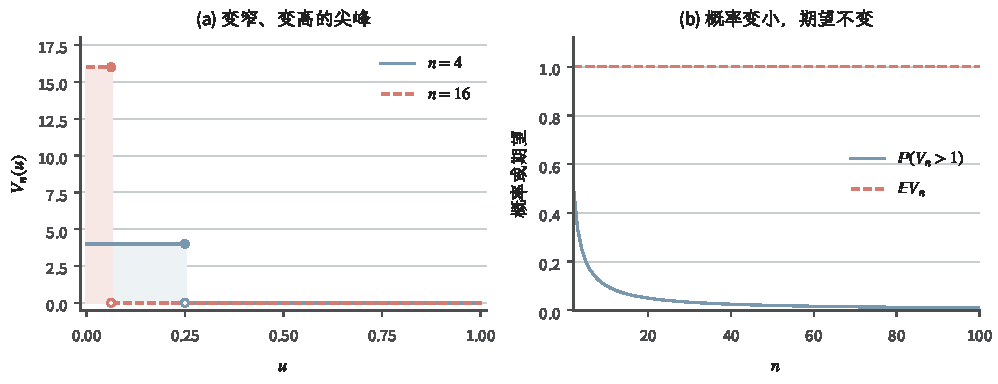
\includegraphics[width=\linewidth]{figures/math-preparation/concept-revision-probability/probability-vanishing-spikes.pdf}
  \caption{小概率尖峰与期望质量（解析式教学图）。左图为\(V_n(u)=n\mathbb I\{u\leq1/n\}\)在\(n=4,16\)时的取值，均以面积\(1\)贡献期望；右图对\(n\geq2\)显示\(\mathbb P(V_n>1)=1/n\)趋于零，而\(\mathbb E V_n=1\)不变。基础变量为\(U\sim\operatorname{Unif}(0,1)\)。}
  \label{fig:probability-vanishing-spikes}
\end{figure*}

\subsubsection{大数定律与样本平均}

\begin{theorem}[强大数定律]
\label{thm:probability-strong-law-large-numbers}
若\(X_1,X_2,\ldots\)独立同分布，且\(\mathbb{E}[|X_1|]<\infty\)，则
\[ \overline{X}_n
  =\frac{1}{n}\sum_{i=1}^{n}X_i\to_{\mathrm{a.s.}}\mathbb{E}[X_1]. \]
\end{theorem}

强大数定律说明同一分布下的独立重复观测，其平均几乎必然接近期望。有限方差是许多初等证明使用的方便条件，但独立同分布版本的结论只需有限一阶绝对矩。若观测相关、分布随
时间变化或样本由自适应规则收集，则不能直接引用该定理；第~\ref{chap:stochastic-processes-and-approximation}章将给出相关过程所需的替代条件
\scite{math-kallenberg2021probability}

有限方差时，较弱的依概率结论可以在这里完整得到。若
\(\operatorname{Var}(X_1)=\sigma^2<\infty\)，独立性使
\[
  \operatorname{Var}(\overline{X}_n)
  =\frac{1}{n^2}\sum_{i=1}^{n}\operatorname{Var}(X_i)
  =\frac{\sigma^2}{n}.
\]
把式~\eqref{eq:probability-chebyshev-inequality}用于样本平均，有
\[
  \mathbb{P}\bigl(
    |\overline{X}_n-\mathbb{E}X_1|\geq\varepsilon
  \bigr)
  \leq\frac{\sigma^2}{n\varepsilon^2}\to0.
\]
这证明了有限方差版本的弱大数定律。强大数定律只要求有限一阶绝对矩，但其证明还需截断大取值、控制截断变量的独立和，并把可求和坏事件转成几乎必然结论；不能由上面的逐个\(n\)概率界直接推出。

对例~\ref{ex:probability-noisy-observation}中的独立同分布噪声，只要\(\mathbb{E}|\varepsilon_i|<\infty\)，便有
\[ \overline{Y}_n
  =\theta+\frac{1}{n}\sum_{i=1}^{n}\varepsilon_i\to_{\mathrm{a.s.}}\theta. \]
这回答了“多测几次再平均是否稳定”，但没有给出固定\(n\)时误差超过指定阈值的概率。

\subsubsection{中心极限定理与缩放波动}

\begin{theorem}[Lindeberg--L\'evy中心极限定理]
\label{thm:probability-iid-central-limit}
若\(X_1,X_2,\ldots\)独立同分布，\(\mathbb{E}X_1=\mu\)，\(0<\operatorname{Var}(X_1)=\sigma^2<\infty\)，则
\[ \frac{\sqrt{n}(\overline{X}_n-\mu)}{\sigma}
  \Rightarrow\mathcal{N}(0,1). \]
\end{theorem}

大数定律研究未缩放误差是否趋于零，中心极限定理研究乘以\(\sqrt{n}\)后的剩余波动近似什么分布。它给出渐近近似，而不是每个有限\(n\)都精确服从高斯分布。若方差
无限、样本依赖过强或分布随\(n\)变化而不满足相应Lindeberg条件，\(\sqrt{n}\)缩放与高斯极限都可能失效。

证明的关键是特征函数。令\(Y_i=(X_i-\mu)/\sigma\)，并记
\(\varphi(t)=\mathbb{E}e^{\mathrm{i}tY_1}\)。复指数绝对值恒为\(1\)，所以特征函数总有定义。由
\(\mathbb{E}Y_1=0\)、\(\mathbb{E}Y_1^2=1\)及零点处的二阶展开，
\[
  \varphi(u)=1-\frac{u^2}{2}+o(u^2),
  \qquad u\to0.
\]
独立性使标准化和的特征函数分解为
\[
  \mathbb{E}\exp\left\{
    \mathrm{i}t\frac{1}{\sqrt n}\sum_{i=1}^{n}Y_i
  \right\}
  =
  \left[\varphi\left(\frac{t}{\sqrt n}\right)\right]^n
  \longrightarrow e^{-t^2/2}.
\]
右侧是标准高斯的特征函数，并且在零点连续。定理
~\ref{thm:probability-levy-continuity}于是给出依分布收敛。第
~\ref{chap:mathematical-statistics}章会用这个渐近分布构造近似区间，但有限样本覆盖
仍需额外误差控制，不能只引用极限式。

\subsection{蒙特卡洛平均与方差控制}
\label{sec:probability-monte-carlo-variance-reduction}

\subsubsection{直接蒙特卡洛估计}

目标积分可统一写成
\[ I=\mathbb{E}_P[f(X)]. \]
若能独立采样\(X_i\sim P\)，直接蒙特卡洛估计为
\[ \widehat{I}_n
  =\frac{1}{n}\sum_{i=1}^{n}f(X_i). \]
当\(\mathbb{E}_P|f(X)|<\infty\)时，大数定律给出一致性；当方差\(\sigma_f^2<\infty\)时，
\[ \operatorname{Var}(\widehat{I}_n)=\frac{\sigma_f^2}{n},
  \qquad\sqrt{n}(\widehat{I}_n-I)\Rightarrow\mathcal{N}(0,\sigma_f^2). \]
误差的标准差按\(n^{-1/2}\)下降，与输入维数没有显式关系，但
\(\sigma_f^2\)可能随问题结构急剧增大。

以下固定教学积分
\[ I=\int_0^1x^2\,\mathrm{d}x=\frac13. \]
若\(X\sim\operatorname{Unif}(0,1)\)，直接平均\(X_i^2\)的单样本方差为
\[ \operatorname{Var}(X^2)
  =\frac15-\frac19=\frac{4}{45}. \]

\subsubsection{重要性采样与方差}

若\(P\ll Q\)，权重\(w=\mathrm{d}P/\mathrm{d}Q\)，则
\[ I=\mathbb{E}_Q[w(X)f(X)]. \]
从\(Q\)采样得到无偏估计
\begin{equation}
  \widehat{I}^{\mathrm{IS}}_n
  =
  \frac{1}{n}\sum_{i=1}^{n}w(X_i)f(X_i),
  \qquad X_1,\ldots,X_n\text{独立同分布于 }Q.
  \label{eq:probability-importance-sampling}
\end{equation}
无偏性只要求乘积可积；有限方差还要求\(\mathbb{E}_Q[w^2f^2]<\infty\)。

对上述积分，取\(Q\)的密度\(q(x)=2x\)，而\(P\)为均匀分布。除零测点\(x=0\)外，\(w(x)=1/(2x)\)，于是\(w(x)f(x)=x/2\)。单样本方差变为
\[ \mathbb{E}_Q\left[\frac{X^2}{4}\right]-\frac19
  =\frac18-\frac19=\frac{1}{72}, \]
小于直接平均的\(4/45\)。这次改进来自\(Q\)把更多样本放到\(x^2\)贡献较大的区域。
并非任意改变分布都会降低方差；若\(Q\)在重要区域过轻，权重尾部反而会放大误差。

这个例子背后有一个理想基准。对固定的被积函数\(f\)，无偏改写其实不要求整个
\(P\ll Q\)，只要求\(Q\)支配有符号测度\(f\,\mathrm{d}P\)：若\(Q(A)=0\)，则
\(\int_A|f|\,\mathrm{d}P=0\)。当\(P,Q\)相对于同一测度分别有密度\(p,q\)时，这等价于
\(q(x)>0\)在\(|f(x)|p(x)>0\)处几乎处处成立。此时令
\[
  h_Q(x)=\frac{f(x)p(x)}{q(x)},\qquad q(x)>0,
\]
便有\(I=\mathbb{E}_Q[h_Q(X)]\)。若
\(0<\mathbb{E}_P|f(X)|<\infty\)，则在满足这一支配条件的提议密度中，使
\(\mathbb{E}_Q[h_Q^2]\)最小的选择满足
\[
  q^\star(x)
  =
  \frac{|f(x)|p(x)}{\mathbb{E}_P|f(X)|}.
\]
它把采样质量直接放到被积函数绝对贡献大的区域。若\(f(x)=0\)而\(p(x)>0\)，则
\(q^\star(x)=0\)，所以一般并没有\(P\ll Q^\star\)，密度比\(p/q^\star\)也不必在该点
定义；但该点对\(f\,\mathrm{d}P\)没有贡献，而且不会被\(Q^\star\)采到，只需把
\(h_{Q^\star}\)定义到\(Q^\star\)-几乎处处即可。特别地，当\(f\geq0\)时，
\(q^\star=fp/I\)，且\(h_{Q^\star}(X)=I\)在\(Q^\star\)下几乎处处成立，理论方差为零。

这个分布通常不能直接执行：归一化常数就是未知积分\(I\)，而从\(fp/I\)精确采样也可能
与原问题一样困难。若还要用同一组权重估计其他被积函数，因而必须保留\(P\ll Q\)，可以
取\(q_\eta=(1-\eta)q^\star+\eta p\)，其中\(0<\eta<1\)；混入的\(p\)为所有
\(P\)-正质量区域保留严格正支持。理想分布因此只提供设计直觉；实际提议分布还必须能够
归一化、采样并计算密度，同时覆盖\(|f|p\)非零的区域。

\subsubsection{控制变量与相关性}

若辅助变量\(h(X)\)的均值\(\mu_h\)已知，则对任意\(\beta\)，
\[ f_\beta(X)
  =f(X)-\beta(h(X)-\mu_h) \]
仍有期望\(I\)。其方差为
\[ \operatorname{Var}(f_\beta)
  =\operatorname{Var}(f)-2\beta\operatorname{Cov}(f,h)+\beta^2\operatorname{Var}(h). \]
当\(\operatorname{Var}(h)>0\)时，最优系数为
\[ \beta^\star
  =\frac{\operatorname{Cov}(f,h)}{\operatorname{Var}(h)}. \]
对\(f(X)=X^2\)、\(h(X)=X\)与均匀\(X\)，有
\(\mu_h=1/2\)且\(\beta^\star=1\)。调整后的变量
\[ X^2-X+\frac12 \]
仍以\(1/3\)为均值，方差降为\(1/180\)。实际用同一批数据估计\(\beta^\star\)时，有限样本无偏性和方差公式需要重新核对；把估计系数当成固定常数会忽略额外随机性。

\subsubsection{Rao--Blackwell化与方差分解}

设\(Y\)是目标\(I\)的无偏估计，\(\mathbb{E}[Y^2]<\infty\)。对某个统计量\(T\)定义
\[ Y^\star=\mathbb{E}[Y\mid T]. \]
全期望公式给出\(\mathbb{E}Y^\star=I\)，全方差公式给出
\begin{equation}
  \operatorname{Var}(Y)
  =
  \mathbb{E}[\operatorname{Var}(Y\mid T)]
  +
  \operatorname{Var}(Y^\star)
  \geq
  \operatorname{Var}(Y^\star).
  \label{eq:probability-rao-blackwell-variance}
\end{equation}
这就是Rao--Blackwell化：在保持均值的同时，对已知信息求条件平均，消去条件内噪声。

仍以\(I=1/3\)为例。独立生成\(X,U\sim\operatorname{Unif}(0,1)\)，令
\[ Y=\mathbb{I}\{U\leq X^2\}. \]
则\(\mathbb{E}Y=1/3\)，而\(\mathbb{E}[Y\mid X]=X^2\)。因此直接平均\(X^2\)可以看成命中估计\(Y\)关于\(X\)的Rao--Blackwell化，方差从
\((1/3)(2/3)=2/9\)降为\(4/45\)。

\subsubsection{自归一化权重与比值估计}

设\(P\ll Q\)，但只能在未知公共常数倍的意义下计算目标密度比，即对某个\(c>0\)，
\[
  \widetilde{w}(x)
  =
  c\,\frac{\mathrm{d}P}{\mathrm{d}Q}(x),
\]
在\(Q\)-几乎处处意义下成立。对独立同分布样本\(X_i\sim Q\)，在分母为正时使用
\(\widetilde{w}_i=\widetilde{w}(X_i)\)并定义
\begin{equation}
  \widehat{I}^{\mathrm{SN}}_n
  =
  \frac{\sum_{i=1}^{n}\widetilde{w}_if(X_i)}
       {\sum_{i=1}^{n}\widetilde{w}_i}.
  \label{eq:probability-self-normalized-importance-sampling}
\end{equation}
它是两个随机平均的比值，通常在有限样本下有偏，因为一般而言\(\mathbb{E}[A/B]\neq\mathbb{E}A/\mathbb{E}B\)。在适当矩条件和分母极限为正时，大数定律仍可给出一致性。
更具体地，若
\(\mathbb{E}_Q[|\widetilde{w}f|]<\infty\)且
\(0<\mathbb{E}_Q[\widetilde{w}]<\infty\)，则强大数定律给出
\[
  \widehat{I}^{\mathrm{SN}}_n
  \longrightarrow
  \frac{\mathbb{E}_Q[\widetilde{w}f]}
       {\mathbb{E}_Q[\widetilde{w}]}
  =
  \frac{c\mathbb{E}_P[f]}{c}
  =I
  \qquad\text{几乎必然}.
\]
若\(\widetilde{w}\)不是目标密度比的公共常数倍，同一比值仍可能收敛，但极限一般对应另一个归一化加权分布，不能据此声称估计的是
\(\mathbb{E}_P[f]\)。

一个三点分布可以同时看清方差、截断与重采样的不同作用。令支持集为
\(\{a,b,c\}\)，提议分布和目标分布分别为
\[
  Q=(0.8,0.15,0.05),\qquad
  P=(0.4,0.3,0.3),
\]
于是重要性权重为\(w=(0.5,2,6)\)。对
\(f=(0,1,1)\)，目标均值为\(I=0.6\)。原始单样本贡献
\(Z=wf=(0,2,6)\)满足
\[
  \mathbb{E}_Q Z=0.6,\qquad
  \operatorname{Var}_Q(Z)
  =\{0.15\times4+0.05\times36\}-0.6^2
  =2.04.
\]
因此\(n\)个独立样本的无偏估计方差为\(2.04/n\)。若把权重截断在\(2\)，则
\(w^{(2)}=(0.5,2,2)\)，相应贡献的期望变为\(0.4\)，方差变为
\[
  \{0.15\times4+0.05\times4\}-0.4^2=0.64.
\]
截断降低了方差，却引入\(-0.2\)的偏差；两者必须同时报告。

再看一组恰好含\(16\)个\(a\)、\(3\)个\(b\)和\(1\)个\(c\)的二十粒子样本。
原始权重总和为\(20\)，归一化后的三点质量恰为\((0.4,0.3,0.3)\)。按这些质量做
\(20\)次多项重采样，三点后代数的条件期望为\((8,6,6)\)；重采样后无权平均的条件
期望仍为\(0.6\)，但条件方差增加了
\[
  \frac{0.6(1-0.6)}{20}=0.012.
\]
若先截断，归一化质量变成\((0.5,0.375,0.125)\)，重采样均值的条件期望是\(0.5\)，
不会恢复被截断改变的目标。原始和截断权重在这组粒子上的经验有效样本量分别约为
\(400/52=7.69\)与\(256/20=12.8\)：较均匀的权重提高了这一诊断量，但不证明偏差消失。

经验有效样本量常写成
\[ \widehat{n}_{\mathrm{eff}}
  =\frac{(\sum_i\widetilde{w}_i)^2}{\sum_i\widetilde{w}_i^2}. \]
它是权重退化的诊断量，不是对所有估计目标都成立的精确独立样本数。截断权重可降低
方差，却通常引入偏差；重采样减少后续计算中的权重不均，却增加额外随机性。本节的“自归一化”是随机比值估计，第~\ref{sec:stoch-self-normalized-adaptive-design}节的自归一化集中则用随机设计矩阵度量累计噪声，二者对象不同。

\subsection{尾部概率与集中不等式}
\label{sec:probability-concentration-inequalities}

\subsubsection{Chernoff方法与指数矩}

对任意\(\lambda>0\)，函数\(x\mapsto e^{\lambda x}\)单调。Markov不等式给出
\begin{equation}
  \mathbb{P}(X\geq t)
  =
  \mathbb{P}(e^{\lambda X}\geq e^{\lambda t})
  \leq
  e^{-\lambda t}\mathbb{E}[e^{\lambda X}].
  \label{eq:probability-chernoff-step}
\end{equation}
随后对\(\lambda\)优化，便得到Chernoff方法。整个方法依赖相应指数矩有限；若\(\mathbb{E}e^{\lambda X}=\infty\)，式
\eqref{eq:probability-chernoff-step}虽形式上仍真，却不给出有用上界。

\begin{definition}[次高斯变量]
  \label{def:probability-subgaussian}
对\(\sigma^2>0\)，均值为零的可积实随机变量\(X\)若满足
\[ \mathbb{E}[e^{\lambda X}]
  \leq\exp\left(\frac{\lambda^2\sigma^2}{2}\right),\qquad \lambda\in\mathbb{R}, \]
就称它为参数\(\sigma^2\)的\term{次高斯变量}（sub-Gaussian random variable）。
\end{definition}
代入Chernoff界并取\(\lambda=t/\sigma^2\)，得到
\[ \mathbb{P}(X\geq t)
  \leq\exp\left(-\frac{t^2}{2\sigma^2}\right). \]
“次高斯”描述的是指数矩或尾部上界，不表示变量本身服从高斯分布。

\subsubsection{有界变量的Hoeffding不等式}

\begin{lemma}[Hoeffding引理]
\label{lem:probability-hoeffding-lemma}
若\(\mathbb{E}X=0\)且\(X\in[a,b]\)几乎处处成立，则
\[ \mathbb{E}[e^{\lambda X}]
  \leq\exp\left\{\frac{\lambda^2(b-a)^2}{8}\right\},\qquad \lambda\in\mathbb{R}. \]
\end{lemma}

\begin{proof}
凸性说明，对\(x\in[a,b]\)，指数函数位于连接端点的弦下方：
\[ e^{\lambda x}
  \leq\frac{b-x}{b-a}e^{\lambda a}+\frac{x-a}{b-a}e^{\lambda b}. \]
取期望并使用\(\mathbb{E}X=0\)，右侧成为一个只依赖
\(\lambda(b-a)\)与均值位置的二点分布矩母函数。令\(p=-a/(b-a)\)，对其对数作二阶导数，可得二阶导数至多为\(1/4\)；该对数在
\(\lambda=0\)处的函数值和一阶导数均为零。两次积分于是给出
\[ \log\mathbb{E}[e^{\lambda X}]
  \leq\frac{\lambda^2(b-a)^2}{8}. \]
指数化即得结论。
\end{proof}

\begin{theorem}[Hoeffding不等式]
\label{thm:probability-hoeffding-inequality}
设\(X_1,\ldots,X_n\)相互独立，且\(X_i\in[a_i,b_i]\)几乎处处成立。则对\(t>0\)，
\[
  \mathbb{P}\left(
    \sum_{i=1}^{n}(X_i-\mathbb{E}X_i)\geq t
  \right)
  \leq
  \exp\left\{
    -\frac{2t^2}{\sum_{i=1}^{n}(b_i-a_i)^2}
  \right\}.
\]
\end{theorem}

\begin{proof}
记\(S=\sum_i(X_i-\mathbb{E}X_i)\)。对\(\lambda>0\)，独立性使指数矩分解：
\[
\begin{aligned}
  \mathbb{P}(S\geq t)
  &\leq
  e^{-\lambda t}\mathbb{E}[e^{\lambda S}]\\
  &=
  e^{-\lambda t}
  \prod_{i=1}^{n}
  \mathbb{E}\left[
    e^{\lambda(X_i-\mathbb{E}X_i)}
  \right]\\
  &\leq
  \exp\left\{
    -\lambda t+
    \frac{\lambda^2}{8}
    \sum_{i=1}^{n}(b_i-a_i)^2
  \right\}.
\end{aligned}
\]
右侧关于\(\lambda\)的最小点为
\[ \lambda^\star
  =\frac{4t}{\sum_i(b_i-a_i)^2}. \]
代回即得结论。对\(-S\)使用同一结果，再用联合界可得双侧版本。
\end{proof}

若\(X_i\in[0,1]\)独立，则样本平均满足
\[ \mathbb{P}(|\overline{X}_n-\mathbb{E}\overline{X}_n|
  \geq\varepsilon)\leq 2e^{-2n\varepsilon^2}. \]
有界性进入Hoeffding引理，独立性进入矩母函数乘积；删除任一条件都不能沿用这份证明。

\subsubsection{方差敏感的Bernstein不等式}

若独立中心化变量满足\(|X_i|\leq M\)，并记\(v=\sum_i\mathbb{E}[X_i^2]\)，则Bernstein不等式的一个版本为
\begin{equation}
  \mathbb{P}\left(\sum_{i=1}^{n}X_i\geq t\right)
  \leq
  \exp\left\{
    -\frac{t^2}{2(v+Mt/3)}
  \right\}.
  \label{eq:probability-bernstein-inequality}
\end{equation}
为看清两个尺度的来源，取\(0<\lambda<3/M\)。由指数级数及
\(|X_i|^k\leq M^{k-2}X_i^2\)（\(k\geq2\)），有
\[
  \mathbb{E}e^{\lambda X_i}
  \leq
  1+\frac{\lambda^2\mathbb{E}X_i^2}
           {2(1-\lambda M/3)}
  \leq
  \exp\left\{
    \frac{\lambda^2\mathbb{E}X_i^2}
         {2(1-\lambda M/3)}
  \right\}.
\]
这里第一阶项因中心化而消失，常数\(1/3\)来自用几何级数控制
\[
  \sum_{k\geq3}\frac{(\lambda M)^{k-2}}{k!}.
\]
独立性使各指数矩相乘，Chernoff步骤于是给出
\[
  \mathbb{P}\left(\sum_iX_i\geq t\right)
  \leq
  \exp\left\{
    -\lambda t+\frac{\lambda^2v}
      {2(1-\lambda M/3)}
  \right\}.
\]
取\(\lambda=t/(v+Mt/3)\)便得到式~\eqref{eq:probability-bernstein-inequality}。小偏差区域由\(v\)主导，呈高斯型；大偏差区域由\(Mt\)主导，呈指数型。

例如\(B_i\sim\operatorname{Bernoulli}(0.01)\)独立，考虑
\(\overline{B}_n-0.01\geq0.05\)。Hoeffding上界为
\(\exp(-0.005n)\)，而Bernstein上界约为
\[
  \exp\left\{
    -\frac{0.05^2n}
      {2(0.01\times0.99+0.05/3)}
  \right\}
  \approx \exp(-0.047n).
\]
低发生率使实际方差远小于区间最坏尺度，所以后者明显更紧；当方差接近区间允许的最大值或偏差进入线性尺度时，Bernstein并不保证处处优于Hoeffding。

对重尾变量，方差可能不存在，指数矩也可能对所有正参数发散。此时Chebyshev、Hoeffding和Bernstein各自在矩、范围或指数矩步骤失效。可以增加截断、稳健均值或仅用
有限\(p\)阶矩推导多项式尾界，但所得估计对象和偏差需要重新说明，不能继续声称高斯型集中。

\section{同时控制与重排对称}
\label{sec:probability-uniform-errors-symmetry}

上节主要控制一个预先指定的平均。按数据选择候选时，需要让误差界对所有可能被选中的对象同时成立，
这引出函数类的联合误差。章末再考察另一种保证来源：如果观测重排后联合分布不变，
即使没有独立性，秩也可能给出精确的有限样本覆盖。两条路线依赖不同条件。

\subsection{多个对象与随机函数的联合误差}
\label{sec:probability-random-functions-uniform-error}

\subsubsection{有限候选的一致误差}

设有限候选类\(\mathcal{H}=\{h_1,\ldots,h_M\}\)，损失\(\ell(h,Z)\in[0,1]\)。真实风险与经验风险分别为
\[ R(h)=\mathbb{E}[\ell(h,Z)],
  \qquad\widehat{R}_n(h)=\frac{1}{n}\sum_{i=1}^{n}\ell(h,Z_i), \]
其中\(Z_1,\ldots,Z_n\)独立同分布。对预先固定的单个\(h\)，Hoeffding不等式给出
\[ \mathbb{P}\bigl(
    |\widehat{R}_n(h)-R(h)|>\varepsilon\bigr)\leq 2e^{-2n\varepsilon^2}. \]
但经验最优候选
\(\widehat{h}\in\arg\min_h\widehat{R}_n(h)\)由同一批数据选出，不是预先固定对象。只控制一个候选不能排除“恰好因噪声看起来最好”的选择偏差。

为明确“同时控制”与“样本量足够”的关系，把上述要求写成一个定义。这里讨论抽样前固定的函数类；所有上确界均假定可测。一项常用充分条件是存在可数子类，使每个函数都是该子类中某个序列的逐点极限。
\begin{definition}[分布无关的一致收敛]
  \label{def:uniform-convergence}
  设\(\mathcal G\)是非空的\([0,1]\)值可测函数类。若对任意\(\eta,\delta\in(0,1)\)，存在只依赖\(\mathcal G,\eta,\delta\)的整数\(n_0\)，使任意概率分布\(P\)和任意\(n\geq n_0\)的独立同分布样本\(S=(Z_1,\ldots,Z_n)\sim P^n\)均满足
  \begin{equation}
    \mathbb P_{S\sim P^n}\left\{
      \sup_{g\in\mathcal G}\left|\frac1n\sum_{i=1}^ng(Z_i)-\mathbb E_Pg\right|\leq\eta
    \right\}\geq1-\delta,
    \label{eq:uniform-convergence-definition}
  \end{equation}
  就称\(\mathcal G\)满足分布无关的\term{一致收敛}（uniform convergence）。若只要求\(P\)属于指定分布族，同一定义给出相对于该分布族的一致收敛。
\end{definition}
“函数上一致”由上确界表达，“分布无关”则要求同一个\(n_0\)适用于全部允许分布。对每个固定函数或每个固定分布分别存在的样本量，不能自动满足这两个量词。

\begin{theorem}[有限函数类的一致误差界]
\label{thm:probability-finite-class-uniform-bound}
在上述条件下，对任意\(\delta\in(0,1)\)，以至少\(1-\delta\)的概率同时对所有\(h\in\mathcal{H}\)有
\begin{equation}
  |\widehat{R}_n(h)-R(h)|
  \leq
  \sqrt{\frac{\log(2M/\delta)}{2n}}.
  \label{eq:probability-finite-class-bound}
\end{equation}
\end{theorem}

\begin{proof}
对每个\(h\)定义坏事件
\[ A_h=
  \{|\widehat{R}_n(h)-R(h)|>\varepsilon\}. \]
单函数Hoeffding界给出\(\mathbb{P}(A_h)\leq2e^{-2n\varepsilon^2}\)。由联合界，
\[ \mathbb{P}\left(\bigcup_{h\in\mathcal{H}}A_h\right)
  \leq 2M e^{-2n\varepsilon^2}. \]
令右侧等于\(\delta\)，解得\(\varepsilon=\sqrt{\log(2M/\delta)/(2n)}\)。在坏事件并集的补集上，结论对
全部候选同时成立。
\end{proof}

令\(h^\star\in\arg\min_hR(h)\)，并在式\eqref{eq:probability-finite-class-bound}成立的事件上记右侧为\(\varepsilon_n\)。则
\[
\begin{aligned}
  R(\widehat{h})
  &\leq
  \widehat{R}_n(\widehat{h})+\varepsilon_n\\
  &\leq
  \widehat{R}_n(h^\star)+\varepsilon_n\\
  &\leq
  R(h^\star)+2\varepsilon_n.
\end{aligned}
\]
第二步正是经验最优性的用途。候选数只通过\(\log M\)进入，但若候选类本身由同一数据任意生成，简单地把最终数量代入\(M\)未必合法；需要把生成过程纳入统一控制对象。
例如\(M=100\)、\(n=1000\)、\(\delta=0.05\)时，式~\eqref{eq:probability-finite-class-bound}右侧约为
\[
  \sqrt{\frac{\log 4000}{2000}}\approx0.0644.
\]
这个数同时控制一百个预先固定候选，而不是给每个候选各自提供\(95\%\)保证；后一做法的联合失败概率可能远大于\(5\%\)。

\subsubsection{覆盖数与随机投影}

无限函数类不能直接按元素做联合界。第~\ref{chap:functional-analysis-and-approximation}章建立的取值模式与覆盖数提供两种
有限化方法：若样本上只有有限种损失向量，只需对这些模式联合控制；若每个函数都能由有限\(\varepsilon\)-网中的代表逼近，则先控制网点，再用Lipschitz性质把误差转回
原函数。这里的关键不是形式上把“无限”改写成一个大数字，而是证明离散代表确实控制所需误差度量。

\begin{lemma}[覆盖数的有限网控制]
  \label{lem:probability-covering-finite-net}
  设\((\mathcal{F},d)\)具有有限\(\varepsilon\)-网
  \(\mathcal{N}_\varepsilon\)，其大小为
  \(N(\mathcal{F},d,\varepsilon)\)。若随机过程
  \(\{Z_f:f\in\mathcal{F}\}\)满足
  \[
    |Z_f-Z_g|\leq Ld(f,g)
  \]
  几乎处处对所有\(f,g\)成立，并且相关上确界可测，则对任意\(t>0\)，
  \begin{equation}
    \mathbb{P}\left\{
      \sup_{f\in\mathcal{F}}|Z_f|>t+L\varepsilon
    \right\}
    \leq
    N(\mathcal{F},d,\varepsilon)
    \sup_{f\in\mathcal{F}}\mathbb{P}(|Z_f|>t).
    \label{eq:probability-covering-finite-net}
  \end{equation}
\end{lemma}

\begin{proof}
对每个\(f\)选取满足\(d(f,g_f)\leq\varepsilon\)的
\(g_f\in\mathcal{N}_\varepsilon\)。则
\[
  |Z_f|\leq |Z_{g_f}|+L\varepsilon,
\]
所以左侧坏事件包含在
\(\bigcup_{g\in\mathcal{N}_\varepsilon}\{|Z_g|>t\}\)中。对这个有限并集使用联合界
即得结论。
\end{proof}

若\(Z_f=\widehat R_n(f)-R(f)\)，且经验风险与真实风险各自关于\(d\)都是
\(L_0\)-Lipschitz，则引理中的过程常数是\(2L_0\)。因此，网格大小、离散误差
\(2L_0\varepsilon\)和单点尾界必须一起进入结论；只报告覆盖数而不验证Lipschitz传递
还不能控制原函数类。

下面的随机投影会把范数失真化成高斯平方和。
\begin{definition}[卡方分布]
  \label{def:probability-chi-square-distribution}
若\(G_1,\ldots,G_k\)相互独立且都服从标准高斯分布\(\mathcal N(0,1)\)，则称
\[
  Z=\sum_{j=1}^{k}G_j^2
\]
服从自由度为\(k\)的\term{卡方分布}（chi-square distribution），记为
\(Z\sim\chi_k^2\)，其中\(k\)为正整数。
\end{definition}
这个定义也给出后文调用尾界的接口：只要证明一个随机二次量能写成
\(k\)个独立标准高斯的平方和，就可以直接使用下面的结论。

\begin{lemma}[\(\chi^2\)变量的尾界]
  \label{lem:probability-chi-square-tail}
  若\(Z\sim\chi_k^2\)，其中\(k\)为正整数，则对每个\(x>0\)，
  \[
    \mathbb{P}\{Z-k\geq2\sqrt{kx}+2x\}\leq e^{-x},
    \qquad
    \mathbb{P}\{k-Z\geq2\sqrt{kx}\}\leq e^{-x}.
  \]
  因而对\(0<\varepsilon<1\)，
  \begin{equation}
    \mathbb{P}\left(
      \left|\frac{Z}{k}-1\right|>\varepsilon
    \right)
    \leq2\exp\left(-\frac{k\varepsilon^2}{8}\right).
    \label{eq:probability-chi-square-relative-tail}
  \end{equation}
\end{lemma}

\begin{proof}
标准高斯积分给出\(\mathbb E e^{\lambda G^2}=(1-2\lambda)^{-1/2}\)，\(\lambda<1/2\)。独立性因而给出
\[
  \log\mathbb E e^{\lambda(Z-k)}
  =\frac{k}{2}\{-2\lambda-\log(1-2\lambda)\}
  \leq\frac{k\lambda^2}{1-2\lambda},\qquad 0<\lambda<1/2.
\]
最后一步来自\(-u-\log(1-u)=\sum_{j\geq2}u^j/j\leq u^2/[2(1-u)]\)。对上尾使用Chernoff方法，取
\(\lambda=\sqrt{x}/(\sqrt{k}+2\sqrt{x})\)，便在阈值\(2\sqrt{kx}+2x\)处得到指数\(-x\)。
对下尾，用\(u-\log(1+u)\leq u^2/2\)得到
\[
  \log\mathbb E e^{-\lambda(Z-k)}\leq k\lambda^2,\qquad\lambda>0.
\]
取\(\lambda=\sqrt{x/k}\)，在阈值\(2\sqrt{kx}\)处也得到指数\(-x\)。最后取\(x=k\varepsilon^2/8\)。当\(0<\varepsilon<1\)时，两侧阈值均不超过\(k\varepsilon\)，故相对偏差事件包含于对应尾事件的并集，联合界给出式~\eqref{eq:probability-chi-square-relative-tail}。
\end{proof}

现在把单个方向的集中推广到有限点集。这一结果称为Johnson--Lindenstrauss引理：保留有限个距离所需的随机投影维数主要随点数的对数增长，而不由原始坐标数直接决定。
\begin{theorem}[高斯随机投影的距离保持]
  \label{thm:probability-johnson-lindenstrauss}
  给定抽样前固定的\(N\geq2\)个点\(\bm x_1,\ldots,\bm x_N\in\mathbb R^d\)，以及\(\varepsilon,\delta\in(0,1)\)。若\(\bm A\in\mathbb R^{k\times d}\)的元素独立服从\(\mathcal N(0,1/k)\)，且
  \[
    k\geq\frac8{\varepsilon^2}\log\frac{N(N-1)}\delta,
  \]
  则以至少\(1-\delta\)的概率，对全部\(i,j\)同时有
  \begin{equation}
    (1-\varepsilon)\|\bm x_i-\bm x_j\|_2^2
    \leq\|\bm A\bm x_i-\bm A\bm x_j\|_2^2
    \leq(1+\varepsilon)\|\bm x_i-\bm x_j\|_2^2.
    \label{eq:probability-jl-distance-preservation}
  \end{equation}
\end{theorem}
\begin{proof}
固定一个不依赖\(\bm A\)的非零向量\(\bm v\)。矩阵各行独立，每个\((\bm A\bm v)_r\)均为均值零、方差\(\|\bm v\|_2^2/k\)的高斯变量，因此
\[
  \frac{k\|\bm A\bm v\|_2^2}{\|\bm v\|_2^2}\sim\chi_k^2.
\]
引理~\ref{lem:probability-chi-square-tail}使该方向的相对平方范数失真概率不超过\(2e^{-k\varepsilon^2/8}\)。点对差至多有\(N(N-1)/2\)个；对全部非零差使用联合界，失败概率不超过\(N(N-1)e^{-k\varepsilon^2/8}\leq\delta\)。零差经任何线性投影仍为零，无须额外尾界。
\end{proof}
结论控制的是平方距离；对距离本身开方后，因子为\(\sqrt{1\pm\varepsilon}\)。点集须在投影抽样前确定，但在同时保持事件上，可以事后任选这批点中的一对查询。它不保证对观察到\(\bm A\)后任意新造的向量都保持范数；当\(k<d\)时，\(\bm A\)的非零零空间方向就给出反例。这里的常数是便于推导的充分界，也不保证所得\(k\)一定小于\(d\)。

\subsubsection{有界差与数据函数集中}

有些目标不是单个样本平均，而是整个数据集的函数\(F(Z_1,\ldots,Z_n)\)。若替换第\(i\)个输入最多改变\(c_i\)，即
\[ \sup_{\bm{z},z_i'}
  |F(z_1,\ldots,z_i,\ldots,z_n)-F(z_1,\ldots,z_i',\ldots,z_n)|\leq c_i, \]
则独立输入下的McDiarmid不等式给出
\begin{equation}
  \mathbb{P}\bigl(
    F-\mathbb{E}F\geq t
  \bigr)
  \leq
  \exp\left\{
    -\frac{2t^2}{\sum_{i=1}^{n}c_i^2}
  \right\}.
  \label{eq:probability-mcdiarmid}
\end{equation}
其证明把\(F\)依次对前\(i\)个观测条件化，形成Doob鞅；每步有界差控制一个鞅增量，再使用Hoeffding型指数矩界。独立性保证逐步揭示观测时的条件结构，有界差则限制单个观测的影响。

\subsubsection{经验复杂度与随机系数}

有限候选可按数量控制误差；无限类的函数在同一组观测上可能高度相似，直接计数会忽略这种结构。\term{Rademacher复杂度}提供另一种衡量方式：固定观测点后，让函数尽量对齐一组无信号的随机正负号，再对这些正负号平均。能拟合更多随机起伏的类，需要更大的同时误差代价。
\begin{definition}[经验Rademacher复杂度]
  \label{def:rademacher-complexity}
  给定非空实值可测函数类\(\mathcal G\)和样本\(S=(z_1,\ldots,z_n)\)。令\(\sigma_i\)独立且等概率取\(-1,1\)。当上确界可测且期望有限时，\term{经验Rademacher复杂度}定义为
  \begin{equation}
    \widehat{\mathfrak R}_S(\mathcal G)
    =\mathbb E_\sigma\left[\sup_{g\in\mathcal G}\frac1n\sum_{i=1}^n\sigma_i g(z_i)\right].
    \label{eq:empirical-rademacher}
  \end{equation}
\end{definition}
固定的是样本，不是使随机和最大的函数；每一组符号都允许选择不同函数。交换上确界与期望会把所有固定函数的零均值随机和平均成零，丢掉所要衡量的拟合能力。
\begin{definition}[期望Rademacher复杂度]
  \label{def:expected-rademacher-complexity}
  对\(S\sim P^n\)，\term{期望Rademacher复杂度}定义为
  \[
    \mathfrak R_n(\mathcal G)=\mathbb E_{S\sim P^n}\widehat{\mathfrak R}_S(\mathcal G).
  \]
\end{definition}
期望复杂度还平均了抽样结果，故依赖\(P\)；经验复杂度仅依赖给定样本上的函数取值。
允许函数作凸组合会增加候选函数，却未必增加它们对随机符号的最大对齐能力。
原因在于，固定符号后，经验随机和是函数取值的线性泛函：若一个组合的各项都不超过
同一个上界，非负且归一化的加权平均也不能超过它。下面把这一几何性质写成复杂度恒等式。

\begin{theorem}[凸组合的Rademacher复杂度]
\label{thm:ensemble-convex-hull}
设$S=(z_1,\ldots,z_n)$为固定样本，$n\geq1$，$\mathcal B$为非空实值可测函数类，
且在这组样本上统一有界，即存在有限$M$使$|h(z_i)|\leq M$对所有
$h\in\mathcal B$和$i$成立。令
\[
 \operatorname{conv}(\mathcal B)
 =\left\{\sum_{t=1}^T a_t h_t:
 T\geq1,\ h_t\in\mathcal B,\ a_t\geq0,\ \sum_{t=1}^T a_t=1\right\}
\]
为全部有限凸组合构成的函数类。则
\[
 \widehat{\mathfrak R}_S(\operatorname{conv}(\mathcal B))
 =\widehat{\mathfrak R}_S(\mathcal B).
\]
若样本再按$P^n$抽取，几乎必然满足上述样本有界条件，且相应样本上确界可测、期望有限，
则期望Rademacher复杂度也满足同一恒等式。
\end{theorem}

\begin{proof}
固定一组符号$\bm\sigma$。对任意有限凸组合，由$a_t\geq0$和$\sum_ta_t=1$，
\[
 \begin{aligned}
 \frac1n\sum_{i=1}^n\sigma_i\sum_{t=1}^T a_t h_t(z_i)
 &=\sum_{t=1}^T a_t
    \left(\frac1n\sum_{i=1}^n\sigma_i h_t(z_i)\right)\\
 &\leq\sup_{h\in\mathcal B}\frac1n\sum_{i=1}^n\sigma_i h(z_i).
 \end{aligned}
\]
因此凸包上的上确界不超过基类上的上确界。反向不等式来自
$\mathcal B\subseteq\operatorname{conv}(\mathcal B)$：取$T=1$即可得到任意基函数。
于是每一组符号下的两个上确界都相等。样本上的统一有界性保证随机和与其上确界有限，
对$\bm\sigma$取期望便得经验复杂度恒等式；在额外的抽样可测性与可积条件下，再对$S$
取期望即得期望复杂度结论。证明不要求函数类有限，也不要求上确界由某个函数达到。
\end{proof}

例如，只含常值函数$0$和$1$的基类，其凸包包含全部常值$c\in[0,1]$。
固定一个观测点时，正号下的最大随机和为$1$，负号下为$0$，两类的经验复杂度都为
$1/2$。候选函数从两个增加到无穷多个，但线性随机和的最坏值仍由端点决定。
这一定理只控制实值函数的随机线性和；把组合再作阈值化等非线性变换后，
需要另外分析变换后的函数类。非负性与归一化也是凸组合的条件，不能用同一等式处理
任意符号或任意尺度的线性组合。

\begin{definition}[经验高斯复杂度]
  \label{def:gaussian-complexity}
  将随机符号换成独立标准高斯系数\(\xi_i\sim\mathcal N(0,1)\)，定义
  \[
    \widehat{\mathfrak G}_S(\mathcal G)
    =\mathbb E_\xi\left[\sup_{g\in\mathcal G}\frac1n\sum_{i=1}^n\xi_i g(z_i)\right].
  \]
  相应期望高斯复杂度为\(\mathfrak G_n(\mathcal G)=\mathbb E_S\widehat{\mathfrak G}_S(\mathcal G)\)。
\end{definition}
高斯系数的符号与幅度都变化，Rademacher系数只有符号变化。二者是关于函数类的随机平均，不能按某一组系数的最大值直接比较。

双侧误差的证明常使用带绝对值版本
\[
  \widehat{\mathfrak R}^{\mathrm{abs}}_S(\mathcal G)
  =\mathbb E_\sigma\sup_{g\in\mathcal G}\left|\frac1n\sum_i\sigma_i g(z_i)\right|
  =\widehat{\mathfrak R}_S(\mathcal G\cup(-\mathcal G)),
\]
高斯版本同样定义。只有当\(\mathcal G=-\mathcal G\)时，两种约定才可直接等同。例如只含常数函数\(g\equiv1\)的类，其不带绝对值复杂度为\(0\)；带绝对值复杂度为\(n^{-1}\mathbb E|\sum_i\sigma_i|>0\)。以下对称化沿用带绝对值约定，后续应用单侧风险界时应核对所用版本。

\subsubsection{对称化与随机函数复杂度}

设\(\mathcal{F}\)是一族取值于\([-1,1]\)的函数，定义
\[ \Delta(\bm{Z})
  =\sup_{f\in\mathcal{F}}\left|\mathbb{E}f(Z)-\frac{1}{n}\sum_{i=1}^{n}f(Z_i)\right|. \]
引入独立同分布副本\(Z_1',\ldots,Z_n'\)。Jensen不等式给出
\[
\begin{aligned}
  \mathbb{E}_{\bm{Z}}\Delta(\bm{Z})
  &\leq
  \mathbb{E}_{\bm{Z},\bm{Z}'}
  \sup_{f\in\mathcal{F}}
  \left|
    \frac{1}{n}\sum_{i=1}^{n}
    \bigl(f(Z_i')-f(Z_i)\bigr)
  \right|.
\end{aligned}
\]
由于每对\((Z_i,Z_i')\)交换后联合分布不变，引入独立Rademacher符号\(\sigma_i\in\{-1,1\}\)不会改变差的联合分布。因此
\[
  \mathbb{E}\Delta(\bm{Z})
  \leq
  2\mathbb{E}_{\bm{Z},\bm{\sigma}}
  \sup_{f\in\mathcal{F}}
  \left|
    \frac{1}{n}\sum_{i=1}^{n}\sigma_i f(Z_i)
  \right|.
\]
右侧是带绝对值的经验Rademacher复杂度对样本取期望后的两倍。它只在观测点上考察函数类与随机符号对齐的能力，把未知总体期望转成了条件于样本的随机和。

若\(\phi_i:\mathbb{R}\to\mathbb{R}\)均为\(L\)-Lipschitz且\(\phi_i(0)=0\)，则对任意不必关于取负封闭的函数类\(\mathcal{F}\)，带绝对值的收缩不等式为
\[
  \mathbb{E}_{\bm{\sigma}}
  \sup_{f\in\mathcal{F}}
  \left|
    \sum_i\sigma_i\phi_i(f(Z_i))
  \right|
  \leq
  2L\,
  \mathbb{E}_{\bm{\sigma}}
  \sup_{f\in\mathcal{F}}
  \left|
    \sum_i\sigma_i f(Z_i)
  \right|.
\]
一般情形需要先在取值向量类中临时加入零向量，再分别控制随机和的两个方向；这一步产生因子\(2\)。若变换后的取值向量类关于取负封闭，例如
\(\mathcal{F}=-\mathcal{F}\)且每个\(\phi_i\)都是奇函数，则可去掉该因子。这个不等式允许把预测函数的复杂度传到Lipschitz损失。若损失不全局Lipschitz或相关上确界不可积，必须限制作用范围或使用其他矩条件。

标量收缩可用逐坐标替换证明。先设函数类在固定样本上的取值向量组成有限集
\(\mathcal{A}\subset\mathbb{R}^n\)，并只考虑不带绝对值的上确界。固定前
\(n-1\)个符号，把相应部分记为\(U_{\bm{a}}\)。条件于这些符号，左侧最后一个坐标的贡献为
\[
  \frac12\sup_{\bm{a}}\{U_{\bm{a}}+\phi_n(a_n)\}
  +\frac12\sup_{\bm{a}}\{U_{\bm{a}}-\phi_n(a_n)\}.
\]
取两个上确界的近似最大元\(\bm{a},\bm{b}\)，并使用
\(\phi_n(a_n)-\phi_n(b_n)\leq L|a_n-b_n|\)。按
\(a_n-b_n\)的符号选择正负方向，便得到上式不超过
\[
  \frac12\sup_{\bm{a}}\{U_{\bm{a}}+La_n\}
  +\frac12\sup_{\bm{a}}\{U_{\bm{a}}-La_n\}.
\]
从最后一个坐标向前迭代，即得到单侧收缩。对随机和的正、负两个方向分别应用该结论，再用
\(\sup|S|=\max\{\sup S,\sup(-S)\}\)时，还需要保证两个单侧上确界非负。具体地，令
\(\mathcal{A}_0=\mathcal{A}\cup\{\bm{0}\}\)。由于\(\phi_i(0)=0\)，对每组固定符号都有
\[
\begin{aligned}
  \sup_{\bm{a}\in\mathcal{A}}
  \left|\sum_i\sigma_i\phi_i(a_i)\right|
  &\leq
  \sup_{\bm{a}\in\mathcal{A}_0}
  \sum_i\sigma_i\phi_i(a_i)
  +
  \sup_{\bm{a}\in\mathcal{A}_0}
  \left(-\sum_i\sigma_i\phi_i(a_i)\right).
\end{aligned}
\]
两个单侧上确界因包含零向量而非负。分别对\(\bm{\sigma}\)与\(-\bm{\sigma}\)应用单侧收缩，再利用二者同分布，得到
\[
  \mathbb{E}_{\bm{\sigma}}
  \sup_{\bm{a}\in\mathcal{A}}
  \left|\sum_i\sigma_i\phi_i(a_i)\right|
  \leq
  2L\,
  \mathbb{E}_{\bm{\sigma}}
  \sup_{\bm{a}\in\mathcal{A}_0}
  \sum_i\sigma_i a_i
  \leq
  2L\,
  \mathbb{E}_{\bm{\sigma}}
  \sup_{\bm{a}\in\mathcal{A}}
  \left|\sum_i\sigma_i a_i\right|.
\]
这就闭合了带绝对值版本的证明。一般函数类可由有限子类逼近并使用单调极限；不可数类还须保留前述可测性条件。

线性函数类展示了这一复杂度怎样落到熟悉的范数上。设
\[
  \mathcal{F}
  =\{\,\bm{z}\mapsto\langle\bm{w},\bm{z}\rangle:
       \lVert\bm{w}\rVert_2\leq B\,\},
  \qquad \lVert\bm{Z}_i\rVert_2\leq R.
\]
由对偶范数和Jensen不等式，
\[
\begin{aligned}
  \widehat{\mathfrak{R}}_{\bm{Z}}^{\mathrm{abs}}(\mathcal{F})
  &=
  \frac{B}{n}\mathbb{E}_{\bm{\sigma}}
  \left\lVert\sum_{i=1}^{n}\sigma_i\bm{Z}_i\right\rVert_2\\
  &\leq
  \frac{B}{n}
  \left(\sum_{i=1}^{n}\lVert\bm{Z}_i\rVert_2^2\right)^{1/2}
  \leq\frac{BR}{\sqrt n}.
\end{aligned}
\]
参数范数、样本范数和样本量分别进入\(B\)、\(R\)与\(n^{-1/2}\)。机器学习理论部分会在具体损失和模型类上继续把这一期望复杂度转换为高概率泛化界。

把Rademacher符号替换为独立标准高斯变量\(g_i\)，得到高斯复杂度
\[ \mathbb{E}_{\bm{g}}
  \sup_{f\in\mathcal{F}}
  \left|\frac{1}{n}\sum_i g_i f(Z_i)\right|. \]
记上述带绝对值的经验Rademacher复杂度和高斯复杂度分别为
\(\widehat{\mathfrak{R}}_{\bm{Z}}^{\mathrm{abs}}(\mathcal{F})\)与
\(\widehat{\mathfrak{G}}_{\bm{Z}}^{\mathrm{abs}}(\mathcal{F})\)。对任意固定样本，只要这些上确界可测且期望有限，就有单向比较
\[
  \widehat{\mathfrak{R}}_{\bm{Z}}^{\mathrm{abs}}(\mathcal{F})
  \leq
  \sqrt{\frac{\pi}{2}}\,
  \widehat{\mathfrak{G}}_{\bm{Z}}^{\mathrm{abs}}(\mathcal{F}).
\]
这个方向可直接由条件Jensen不等式解释：写\(g_i=\sigma_i|g_i|\)，符号与幅度独立，且\(\mathbb E|g_i|=\sqrt{2/\pi}\)。固定符号后，随机和的绝对值上确界是幅度向量的凸函数，先对幅度平均不大于先取上确界再平均，因而\(\widehat{\mathfrak G}^{\mathrm{abs}}_S\geq\sqrt{2/\pi}\,\widehat{\mathfrak R}^{\mathrm{abs}}_S\)。

反方向一般不能只付出普适常数；不附加几何条件时，一个通用界会带
\(O(\sqrt{\log(en)})\)因子。函数类在样本上的取值向量若恰为坐标向量及其相反数，高斯复杂度与
Rademacher复杂度之比就达到\(\Theta(\sqrt{\log n})\)。因此，在泛化界中用一种复杂度替换另一种时，必须保留比较方向及相应因子；高斯过程的协方差度量和覆盖数结构仍需单独估计。

\subsection{可交换性与有限样本秩}
\label{sec:probability-exchangeability-conformal-ranks}

\subsubsection{可交换性与重排对称}

\begin{definition}[可交换随机变量]
  \label{def:probability-exchangeability}
随机变量\(Z_1,\ldots,Z_m\)若对每个排列\(\pi\)都有
\[ (Z_1,\ldots,Z_m)
  \overset{\mathrm{d}}{=}(Z_{\pi(1)},\ldots,Z_{\pi(m)}), \]
就称它们\term{可交换}（exchangeable）。
\end{definition}
独立同分布蕴含可交换，但反向不成立。
例如先抽取随机概率\(\Theta\)，再条件于\(\Theta\)独立生成Bernoulli观测；边缘上这些观测可交换，却因共享\(\Theta\)而相关。

可交换性不提供样本平均的独立乘积结构，因而不能直接代入Hoeffding证明。它提供的是标签位置的对称性：若对全部观测使用同一规则计算分数，则每个分数占据任一秩的位置具有相同机会。共形预测利用的正是这项有限样本对称性。

\subsubsection{秩统计量的对称性}

设实值分数\(S_1,\ldots,S_{m+1}\)可交换，并暂假它们几乎必然没有并列值。令
\[ R_{m+1}
  =1+\sum_{i=1}^{m}\mathbb{I}\{S_i<S_{m+1}\} \]
为最后一个分数从小到大的秩。由于交换任意两个坐标不改变联合分布，而无并列值时每个样本恰占一个秩，所以
\begin{equation}
  \mathbb{P}(R_{m+1}=r)=\frac{1}{m+1},
  \qquad r=1,\ldots,m+1.
  \label{eq:probability-uniform-rank}
\end{equation}
这是一项精确的有限样本结论，不依赖中心极限定理。

若存在并列值，使用“严格小于”的秩不再均匀。可以为每个分数附加独立连续随机数并按字典序打破并列，此时恢复精确均匀秩；也可以采用保守的不随机化分位数，得到覆盖率至少为目标值，但通常不再精确等于目标值。

\subsubsection{拆分共形预测的有限样本覆盖}

设训练数据用于拟合一个固定预测规则，随后有\(m\)个校准样本和一个未来样本。条件于训练数据，假设校准样本与未来样本可交换。用同一个不一致性函数计算
\[ S_i=s(X_i,Y_i),
  \qquad i=1,\ldots,m+1. \]
分数越大表示候选标签与预测规则越不相容。给定错误率\(\alpha\in(0,1)\)，令
\[ k=\left\lceil(m+1)(1-\alpha)\right\rceil. \]
若\(k\leq m\)，令\(q\)为前\(m\)个校准分数的第\(k\)小值；若\(k=m+1\)，约定\(q=+\infty\)。对新输入\(X_{m+1}\)，定义预测集合
\begin{equation}
  C(X_{m+1})
  =
  \{y:s(X_{m+1},y)\leq q\}.
  \label{eq:probability-split-conformal-set}
\end{equation}

例如\(m=9\)、\(\alpha=0.2\)时，\(k=\lceil10\times0.8\rceil=8\)。若排序后的校准分数为
\(0.1,0.2,\ldots,0.9\)，则\(q=0.8\)：候选标签的分数为\(0.75\)时纳入集合，为\(0.85\)时排除。若仍只有九个校准样本却要求
\(\alpha=0.05\)，则\(k=\lceil9.5\rceil=10=m+1\)，按约定得到\(q=+\infty\)。这不是计算故障，而是有限样本不足以用非随机秩给出如此高的非平凡覆盖水平。

\begin{theorem}[拆分共形的有限样本覆盖]
\label{thm:probability-split-conformal-coverage}
在上述条件下，
\[ \mathbb{P}\bigl(
    Y_{m+1}\in C(X_{m+1})\bigr)\geq 1-\alpha. \]
\end{theorem}

\begin{proof}
先假设分数无并列值。若未来真实标签未被覆盖，则\(S_{m+1}>q\)，所以未来分数在全部\(m+1\)个分数中的秩严格大于\(k\)。由式~\eqref{eq:probability-uniform-rank}，
\[ \mathbb{P}(S_{m+1}>q)
  =\mathbb{P}(R_{m+1}>k)=\frac{m+1-k}{m+1}\leq\alpha. \]
取补事件即得覆盖结论。

若有并列值，采用集合定义中的“\(\leq q\)”会把边界并列分数纳入预测集合。相较于随机打破并列后的精确秩，这只会增加覆盖事件，因此同一不等式仍成立。若希望得到更接近
精确的覆盖率，可显式随机化边界并列项，但必须把该随机化纳入算法与概率空间。
\end{proof}

这里的概率保证是\term{边际覆盖}：条件于训练数据后，它仍对随机的校准样本和未来样本共同取平均；若采用随机并列处理，还包括该随机性。解除对训练数据的条件后，总体覆盖率仍至少为
\(1-\alpha\)。但这个结论一般不推出对每个固定输入\(x\)都有
\[
  \mathbb{P}\bigl(
    Y_{m+1}\in C(X_{m+1})
    \mid X_{m+1}=x
  \bigr)
  \geq1-\alpha,
\]
也不自动保证每个群组内都达到同一覆盖率。逐输入、逐群组或时间条件覆盖需要额外结构、假设或专门的校准方法，不能仅由可交换秩推出。

证明依赖两处对称性。训练与校准拆分使评分规则在校准阶段保持固定；校准样本与未来样本可交换，使未来分数的秩没有特殊位置。若反复查看校准误差后修改模型或分数函数，评分规则
已依赖校准标签，条件可交换性可能被破坏。时间序列中的未来点通常也不能与过去点任意重排；自适应收集会让被选中的样本位置携带额外信息。此时失效的是均匀秩步骤，而不是把
分位数索引稍作调整就能修复。\BookSectionRef{sec:reliability-guarantee}
{第二卷“基础、理论和可信性”的“可靠性的保证”节}建立具体预测范围后，将回用这一秩保证。

\section{本章小结}
\label{sec:probability-summary}

概率空间把不确定结果组织为事件测度，随机变量再把结果映射成可积分的数值。Radon--Nikodym导数回答怎样在兼容零集的前提下改变参考分布；条件期望则回答可用信息
增加后，怎样保留每个可识别事件上的平均。前者改变积分所用的测度，后者改变答案允许依赖的\(\sigma\)代数，二者不能混为同一种“加权”。

对带噪观测，期望给出目标，大数定律说明样本平均何时稳定，中心极限定理描述缩放后的渐近波动，集中不等式则直接控制固定样本下的尾部概率。蒙特卡洛、重要性采样、控制变量
和Rao--Blackwell化都估计同一个积分，却分别通过改变采样分布、加入已知平均和消去条件噪声来改变方差；无偏、一致与有限方差需要分别核对。

从有限候选中按数据选择对象时，固定单个候选的误差界不够。联合界给出有限类的同时保证，高斯随机投影据此同时保持预先固定点集的成对距离；对称化与随机复杂度把同时控制扩展到结构化无限类。可交换秩则提供另一条有限样本
路线：它不依赖独立平均，而依赖重排对称。渐近近似、固定样本尾界、函数类同时误差和秩覆盖支持的是不同陈述。下一章将研究观测相关、按过去信息自适应选择以及长期迭代时，这些条件需要怎样改变。
